\documentclass[a4paper, 12pt]{article}
\usepackage{titling}
\usepackage{amsmath, amssymb, physics}
\usepackage{chngpage}
\usepackage{multirow}
\usepackage{graphicx}
\usepackage{titlesec}
\usepackage{fancyhdr}
\usepackage{chngcntr}
\graphicspath{ {figs/} }
\usepackage{indentfirst}
\usepackage{relsize}
\usepackage[margin=3cm]{geometry}
\usepackage{multirow}
\usepackage[table,xcdraw]{xcolor}
\usepackage{hhline}
\usepackage{titletoc}
\usepackage{afterpage}
\usepackage{caption} 
\usepackage{float}
\usepackage{listings}
\captionsetup[table]{skip=10pt}
\usepackage{color} %red, green, blue, yellow, cyan, magenta, black, white
\definecolor{mygreen}{RGB}{28,172,0} % color values Red, Green, Blue
\definecolor{mylilas}{RGB}{170,55,241}

\lstset{language=Matlab,%
    %basicstyle=\color{red},ap
    breaklines=true,%
    morekeywords={matlab2tikz, dsolve},
    keywordstyle=\color{blue},%
    morekeywords=[2]{1}, keywordstyle=[2]{\color{black}},
    identifierstyle=\color{black},%
    stringstyle=\color{mylilas},
    commentstyle=\color{mylilas},%
    showstringspaces=false,%without this there will be a symbol in the places where there is a space
    numbers=left,%
    numberstyle={\tiny \color{black}},% size of the numbers
    numbersep=9pt, % this defines how far the numbers are from the text
    emph=[1]{if, for,end,break},emphstyle=[1]\color{red}, %some words to emphasise
    %emph=[2]{word1,word2}, emphstyle=[2]{style},    
	literate={á}{{\'a}}1
        {ã}{{\~a}}1
        {é}{{\'e}}1
        {ó}{{\'o}}1
        {í}{{\'i}}1
        {ñ}{{\~n}}1
        {¡}{{!`}}1
        {¿}{{?`}}1
        {ú}{{\'u}}1
        {Í}{{\'I}}1
        {Ó}{{\'O}}1
}



\setlength{\droptitle}{-15em}


\pagestyle{fancy}
\fancyhf{}
\fancyhead[L]{Control de un motor de C.C.}
\fancyhead[R]{M. de Miguel}
\fancyfoot[c]{\thepage}

\newcommand\blankpage{%
	\null
	\thispagestyle{empty}%
	\addtocounter{page}{-1}%
	\newpage}

\renewcommand{\figurename}{Figura}
\renewcommand{\contentsname}{Índice}
\renewcommand{\tablename}{Tabla}

\begin{document}
	\begin{titlepage}
		\centering
		\vfill
		\Large{UNIVERSIDAD COMPLUTENSE DE MADRID \\ \textbf{FACULTAD DE CIENCIAS FÍSICAS}}
		\vfill
		\begin{figure}[h!]
			\centering
			
\includegraphics[height=9cm]{figs/cumphysics}
		\end{figure}
		\vfill 
		\large{\textbf{SISTEMAS DINÁMICOS Y REALIMENTACIÓN}}
       \vfill
        \rule [5pt]{15cm}{2pt}\\
		\Huge{\textbf{CONTROL DE UN MOTOR DE CORRIENTE CONTINUA}} \\
		\rule [8pt]{15cm}{2pt}\\
		\vfill
		\vfill
		\vfill
		\vfill
		\vfill
		\large{Mario de Miguel Domínguez\\ 19 de enero de 2024}
		\vfill
		\vfill
		\vfill
		\vfill
		
		\afterpage{\blankpage}
	\end{titlepage}
	
	\makeatletter
	\thispagestyle{empty}
	\addtocounter{page}{-1}
	

	\tableofcontents	
	\thispagestyle{empty}
	\afterpage{\blankpage}
	\newpage
\section*{Introducción}
El presente documento es un recopilatorio de las respuestas a las cuestiones planteadas en todas las secciones del guion de la práctica de control del motor de Sistemas Dinámicos y Realimentación. 
Todos los datos experimentales y los modelos se han obtenido o probado con el motor 02. 
\section{Manejo del motor de continua en lazo abierto}
El propósito de esta sección consiste en la elaboración de un modelo del motor que permita leer los valores esperados de la posición y velocidad a través de encoders, en función de una tensión fija aplicada.
\subsection{Construcción del modelo de manejo sin realimentación (Práctica 1)} 
\subsubsection{Identificación de las partes del motor}
A continuación se incluye una imagen en la que se muestran los diferentes componentes del motor con el que se va a trabajar a lo largo de todas las prácticas.

\begin{enumerate}
	\item Motor EMG30
	\item Placa de desarrollo
	\item Placa de expansión
\end{enumerate}

\begin{figure}[h!]
	\centering
	\includegraphics[height = 7cm]{hardware.png}
	\caption{Hardware}
\end{figure}
\subsubsection{Modelo de Simulink para el manejo en lazo abierto}
Para este modelo se empleará un bloque que simulará el motor, que recibirá dos entradas: una analógica representando la tensión que recibe el motor, y una digital que controlará el sentido de giro del motor. 
A su vez, el motor devolverá dos salidas, representativas de los encoders de posición y velocidad, respectivamente. 
\begin{figure}[h!]
	\centering
	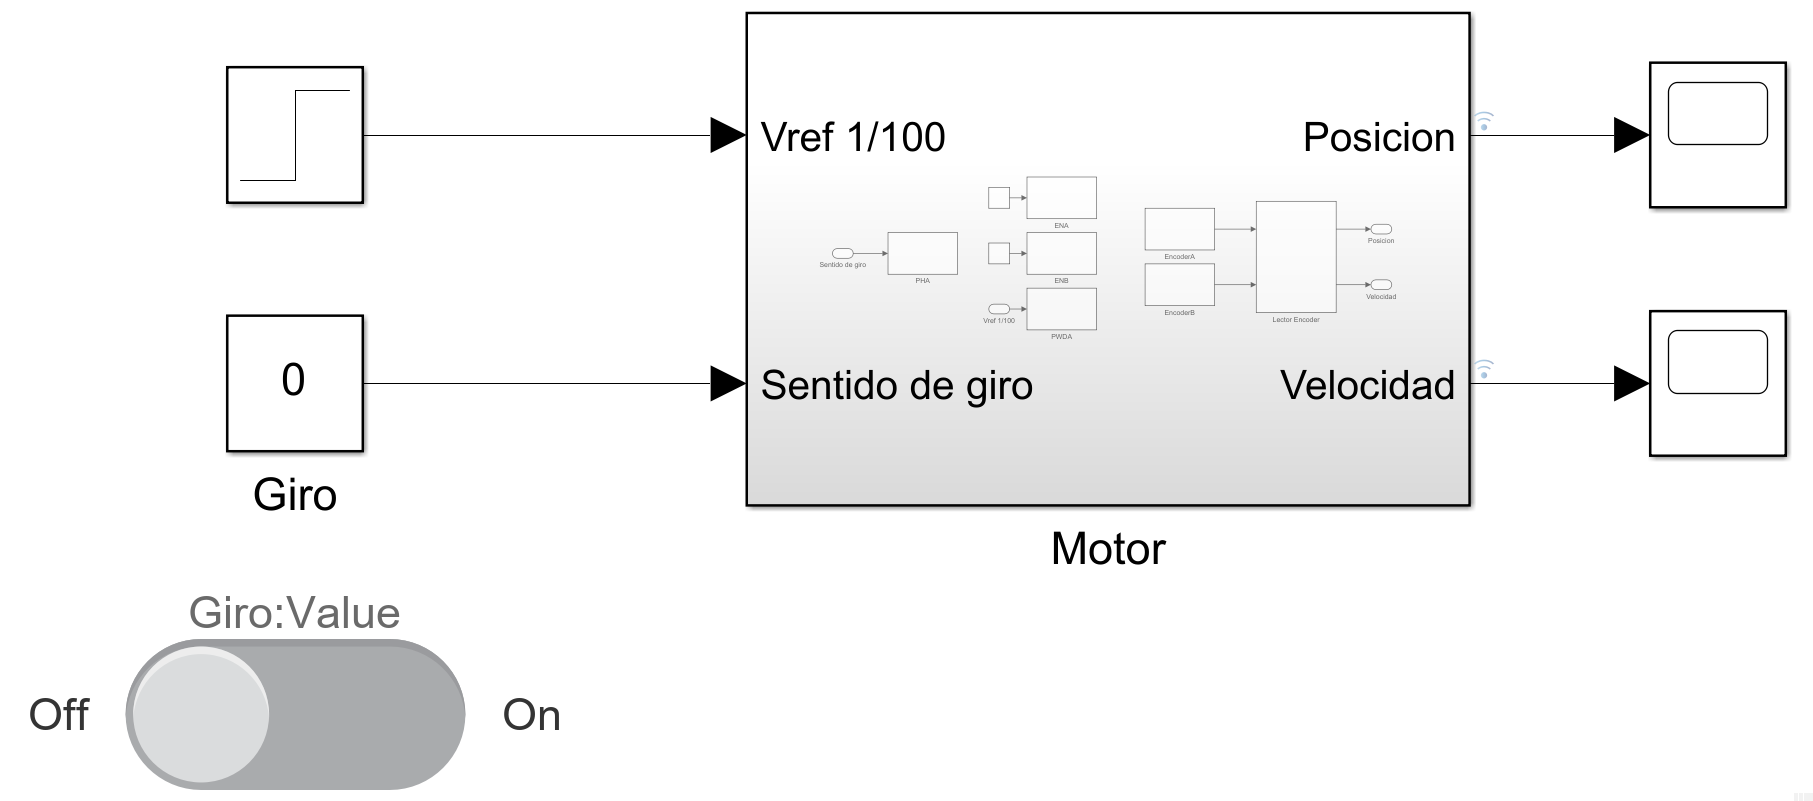
\includegraphics[height=4cm]{figs/motorbb.png}
	\caption{Modelo completo del motor en Simulink}
\end{figure}
\begin{figure}[h!]
	\centering
	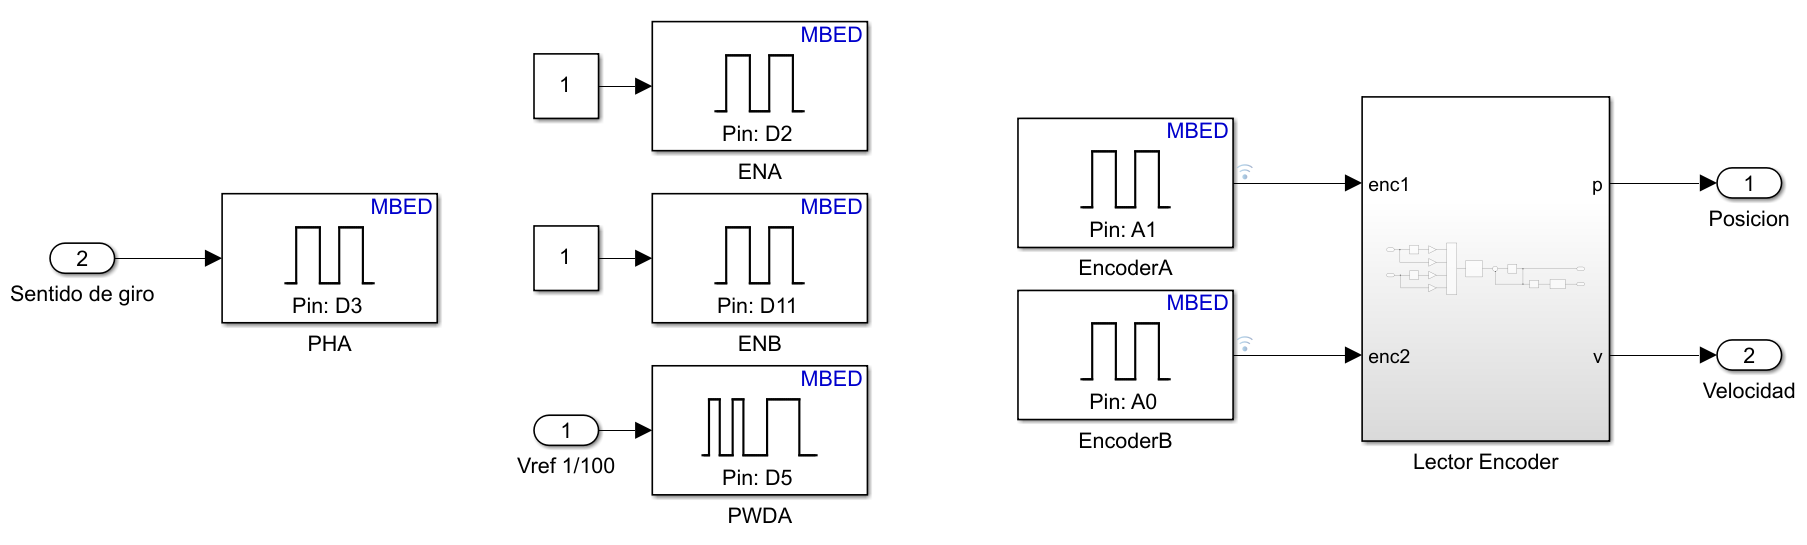
\includegraphics[height = 4cm]{figs/motorbb_inside.png}
	\caption{Bloque del motor}
\end{figure}
\begin{figure}[h!]
	\centering
	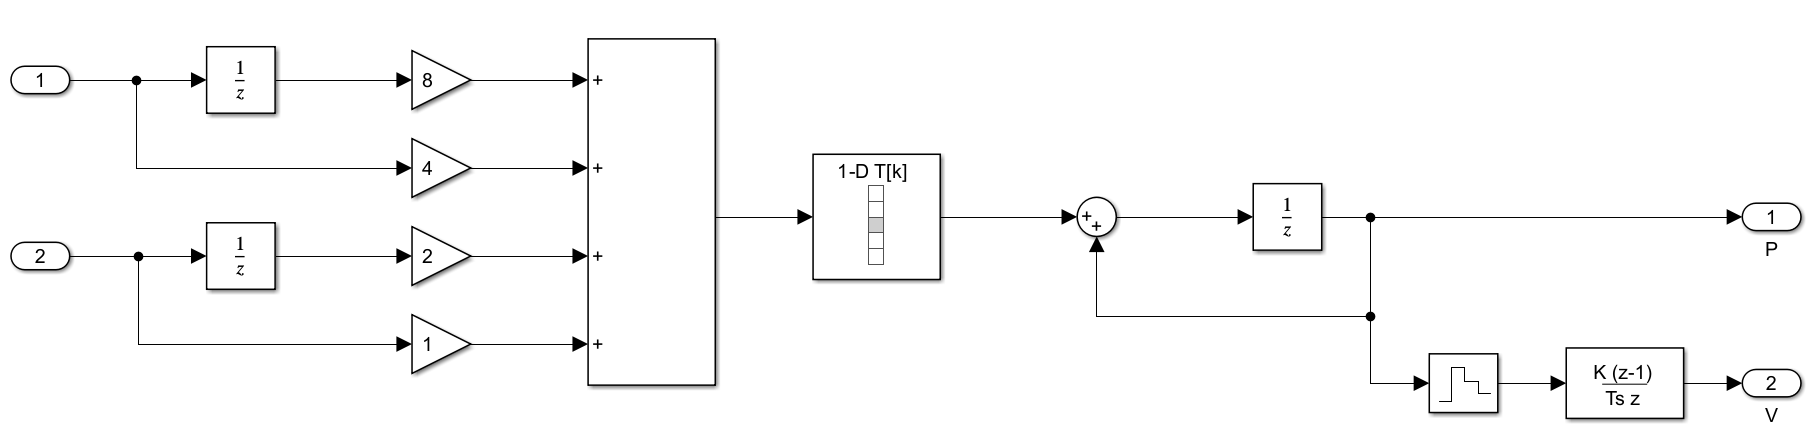
\includegraphics[height = 3.5cm]{figs/lector_encoders.png}
	\caption{Bloque de lectura de los encoders}
\end{figure}

Se observan las señales de los encoders reales del motor (figura \ref{ec}). Como puede verse el resultado no es perfecto, pues hay pulsos que se pierden. Sin embargo, será útil para medir datos de posición, ya que la evolución del sistema es mucho más lenta. Estos fallos en los encoders pueden producir discrepancias de 1º en medidas de posición, lo cual no es un error muy grave. 
\begin{figure}[h!]
	\centering
	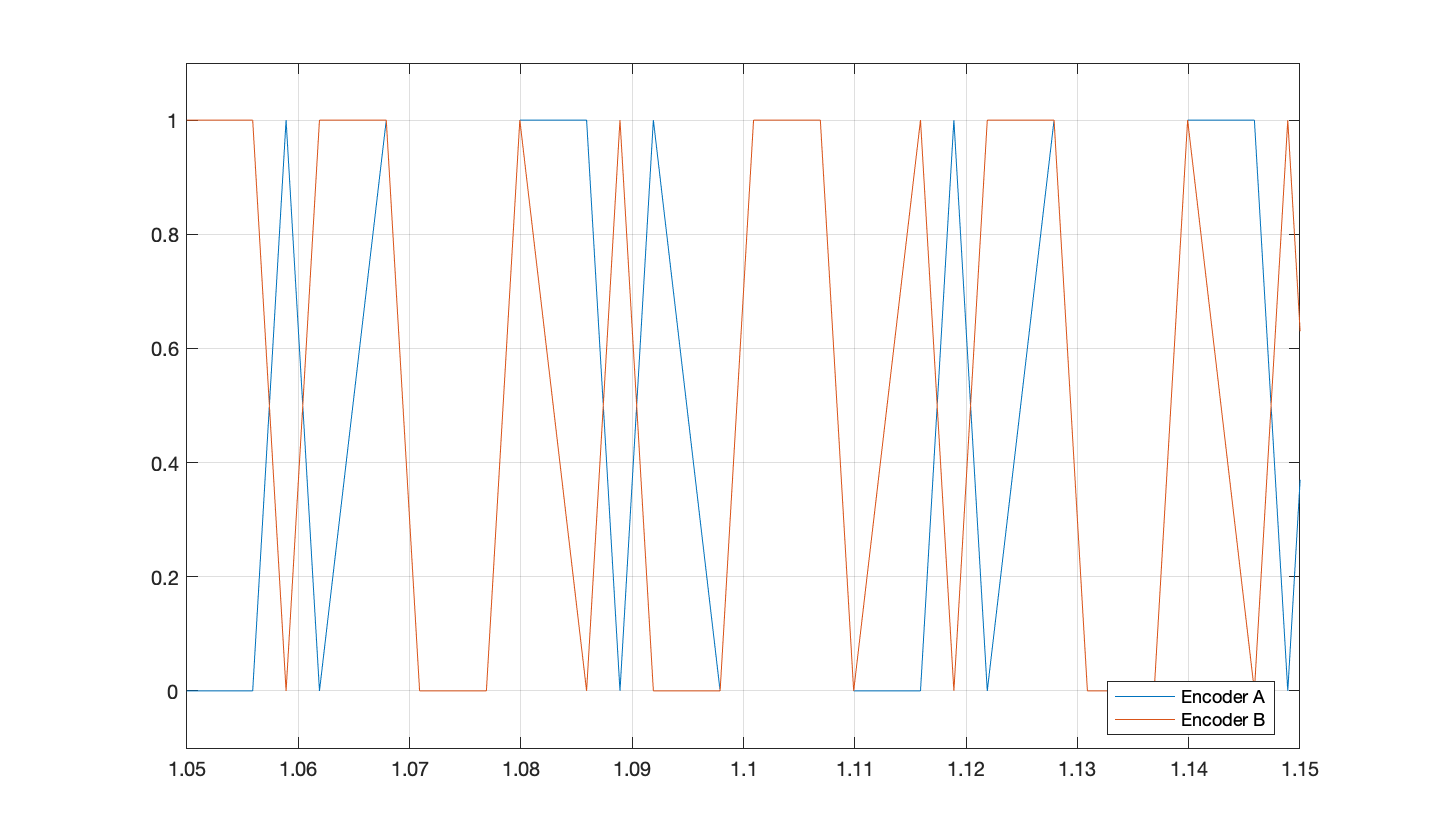
\includegraphics[height = 7.5cm]{p2/encoders}
	\caption{Medida de señal de los encoders para el motor} \label{ec}
\end{figure}

\subsection{Identificación del motor (Práctica 2)} 
\subsubsection{Cálculo de la funciones de respuesta}

A continuación se calcularán las funciones de respuesta de posición y velocidad del motor a partir del modelo en variables de estado y de la función de transferencia. 
Para el modelo en variables de estado, se tiene que 
\begin{align}
	\begin{bmatrix} \dot\theta \\ \dot\omega \end{bmatrix}  =  \begin{bmatrix} 0 & 1 \\ 0 & -p \end{bmatrix} \cdot \begin{bmatrix} \theta \\ \omega  \end{bmatrix} + \begin{bmatrix} 0 \\ k_e \end{bmatrix} V,
\end{align}
de donde se deducen las ecuaciones diferenciales 
\begin{align}
	\dot\theta(t) &= \omega(t) , \label{posdot} \\
	\dot\omega(t) &= -p \omega(t) + k_e V. \label{veldot}
\end{align}

Nótese que hemos definido la tensión de entrada $e(t)$ como una entrada escalón de valor $V$. Basta con resolver las ecuaciones anteriores imponiendo como condición inicial que $\omega(0) = 0, \theta(0) = 0$ para obtener las expresiones de respuesta:
\begin{align}
	\omega(t) &= V\frac{k_e}{p} - \frac{k_e }{p} e^{-p t},  \label{vel}\\
	\theta(t) &= V\frac{k_e}{p^2}e^{-p t} + V\frac{k_e}{p} t - V\frac{k_e}{p^2}.  \label{pos}
\end{align}

Inmediatamente se comprueba que la expresión \ref{pos} es la misma que la ecuación 3.14 del guion. 
Para calcularlo a partir de la función de transferencia de la posición

\begin{equation}
	\theta(s) = \frac{k_e}{s(s + p)} e(s)
\end{equation}
primero hay que calcular la transformada de Laplace de la entrada $e(t) = V$. Como V es una constante, fácilmente se obtiene $e(s) = \mathcal{L} (V) = \frac{V}{s}$. Una vez aplicada esta transformación, se pueden calcular las funciones de respuesta, resultando
\begin{align}
	\theta(t) = \mathcal{L}^{-1} [\theta(s)] &=  \frac{V  k_e }{p} t - \frac{V k_e}{p^2} + \frac{V k_e}{p^2} e^{-p t}, \\
	\omega(t) = \dot\theta(t) &= \frac{V  k_e}{p} - \frac{V k_e}{p} e^{-p t},
\end{align}
que son expresiones idénticas a las obtenidas a partir del modelo en variables de estado (ecuaciones \ref{pos} y \ref{vel}).

\subsubsection{Estimación de los valores de $k_e$ y $p$ del motor}
A continuación se va a tratar de obtener los parámetros del motor utilizando el modelo de Simulink de lazo abierto (Ver sección 1.1.2). 
Para ello, se ha medido la respuesta del motor para varios valores de tensión de entrada (desde 1 a 12 V). Recuperando las ecuaciones \ref{pos} y \ref{vel} y despreciándose el término de exponencial negativa, asumiendo que pierde su influencia muy rápidamente, se puede obtener una regresión lineal de la forma
\begin{equation}\label{poslin}
	\theta(t) \approx \frac{V k_e}{p}t - \frac{V k_e}{p^2} \equiv bt - a
\end{equation}
de manera que 
\begin{align}
	p &= -\frac{b}{a} \\
	k_e &= -\frac{ap^2}{V}.
\end{align}
Un problema que surge al estimar $k_e$ y $p$ por este método es, como el motor no empieza a moverse en el mismo instante en el que se comienza a medir, hay que tener mucho cuidado de empezar a contar muy cerca del instante cuando se empieza a mover para que los valores de $a$ no queden muy desajustados.
Al calcular estos datos para cada tensión, se obtienen los siguientes valores:
\newpage
\begin{table}[hbt!]
	\centering
		\begin{tabular}{ccc}
		$V_{ref}$ & $p$ & $k_e$ \\
		\hline
		1  & -66.9599 & -5000 \\
		2  & 175.1074 & 15380 \\
		3  & 93.6903  & 8838  \\
		4  & 84.9290  & 8265  \\
		5  & 68.1394  & 6681  \\
		6  & 72.9522  & 7266  \\
		7  & 64.6975  & 6511  \\
		8  & 74.1401  & 7468  \\
		9  & 61.8418  & 6273  \\
		10 & 51.2268  & 5226  \\
		11 & 45.8142  & 4669  \\
		12 & 40.0097  & 4101 
		\end{tabular}
		\caption{Valores de identificación del motor}
\end{table}
Estimando las medias de estos valores, se obtiene
\begin{itemize}
	\item $k_e = 7334$ 
	\item $p = 75.69$  
\end{itemize}


Nótese que para realizar esta media se ha descartado el par de valores obtenidos a partir de los datos de $V = 1$, debido a que el cociente entre $k_e$ y $p$ para este valor es muy inferior al resto de resultados, lo que perjudicaría a la media.

\subsubsection{Comparación de los datos reales con el modelo de Simulink}
Se presenta en la siguiente figura un modelo desarrollado en Simulink, incluyendo los parámetros $p$ y $k_e$, construido a partir de las ecuaciones \ref{posdot} y \ref{veldot}. 
\begin{figure}[h!]
	\centering
	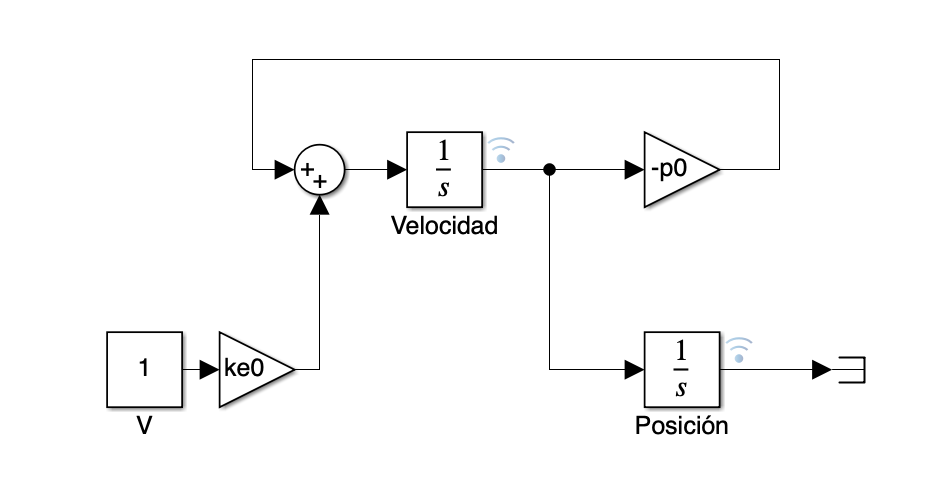
\includegraphics[height=5cm]{figs/pykesimulink}
	\caption{Modelo de Simulink para comprobar los valores obtenidos de $k_e$ y $p$}
\end{figure}

Del anterior modelo se observan las señales de salida de los integradores ``Velocidad" y ``Posición".  Estas salidas se compararán para distintos valores de tensión de entrada con los datos experimentales obtenidos del motor. \\

Seguidamente se grafican estas señales junto a aquellas obtenidas inicialmente del motor para ciertos valores de tensión, por ejemplo 2, 6 y 12 V, 
a fin de observar discrepancias entre ellas. Para valores de 2, 6 y 12 V se obtienen las siguientes gráficas:\\
\begin{figure}[h!] 
	\centering
	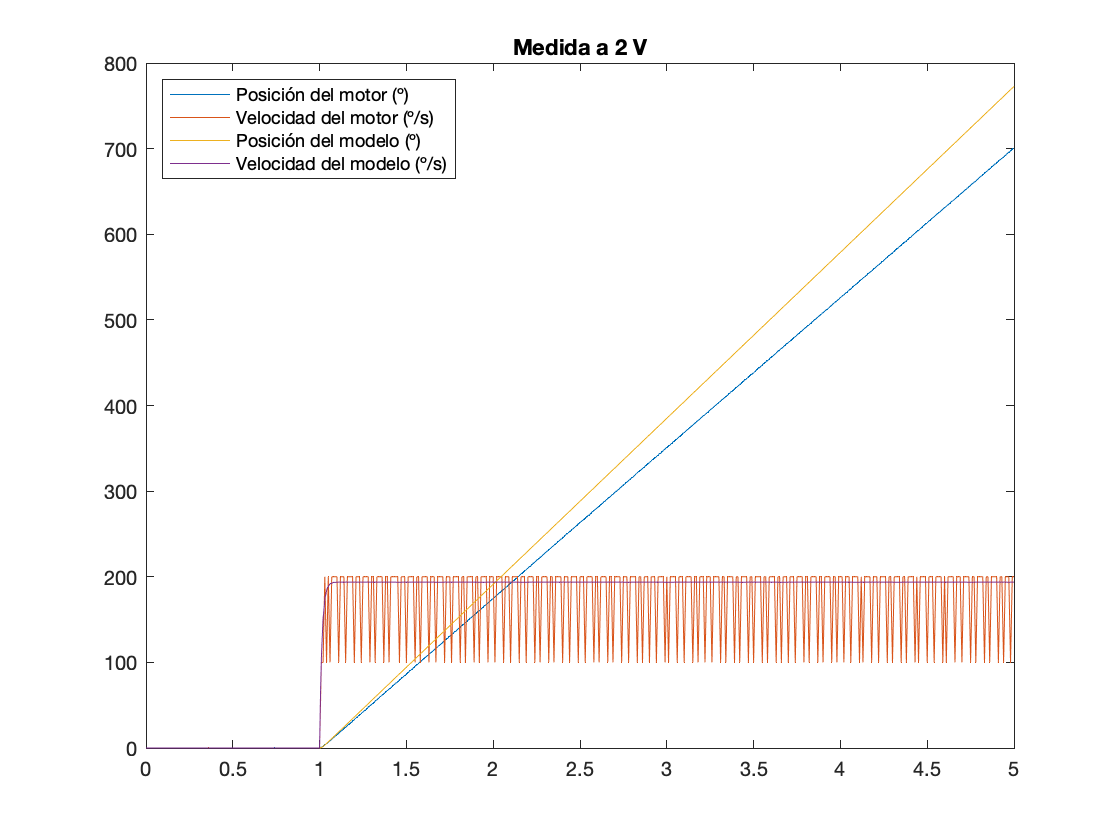
\includegraphics[height=8cm]{figs/p2/v02} 
	\caption{Comparación a 2 V} \label{comp02}
\end{figure}
\begin{figure}[h!]
	\centering
	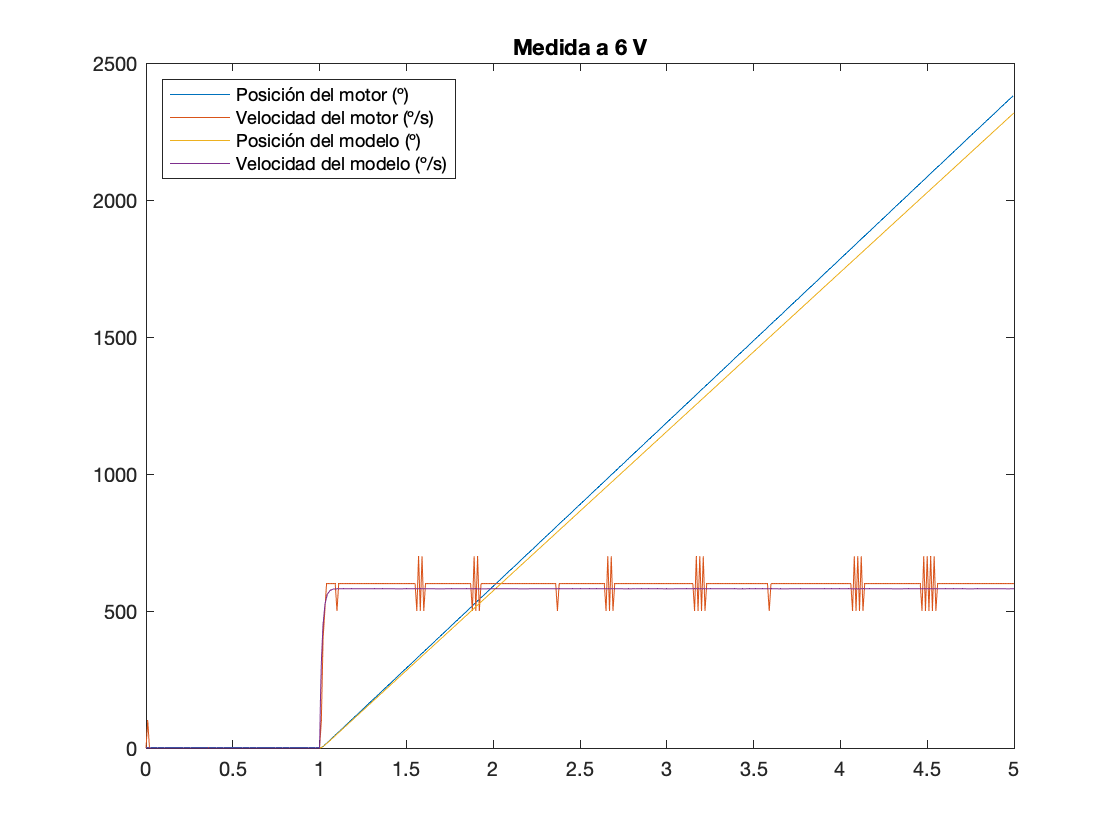
\includegraphics[height=8cm]{figs/p2/v06} 
	\caption{Comparación a 6 V} \label{comp06}
\end{figure}
\begin{figure}[h!]
	\centering
	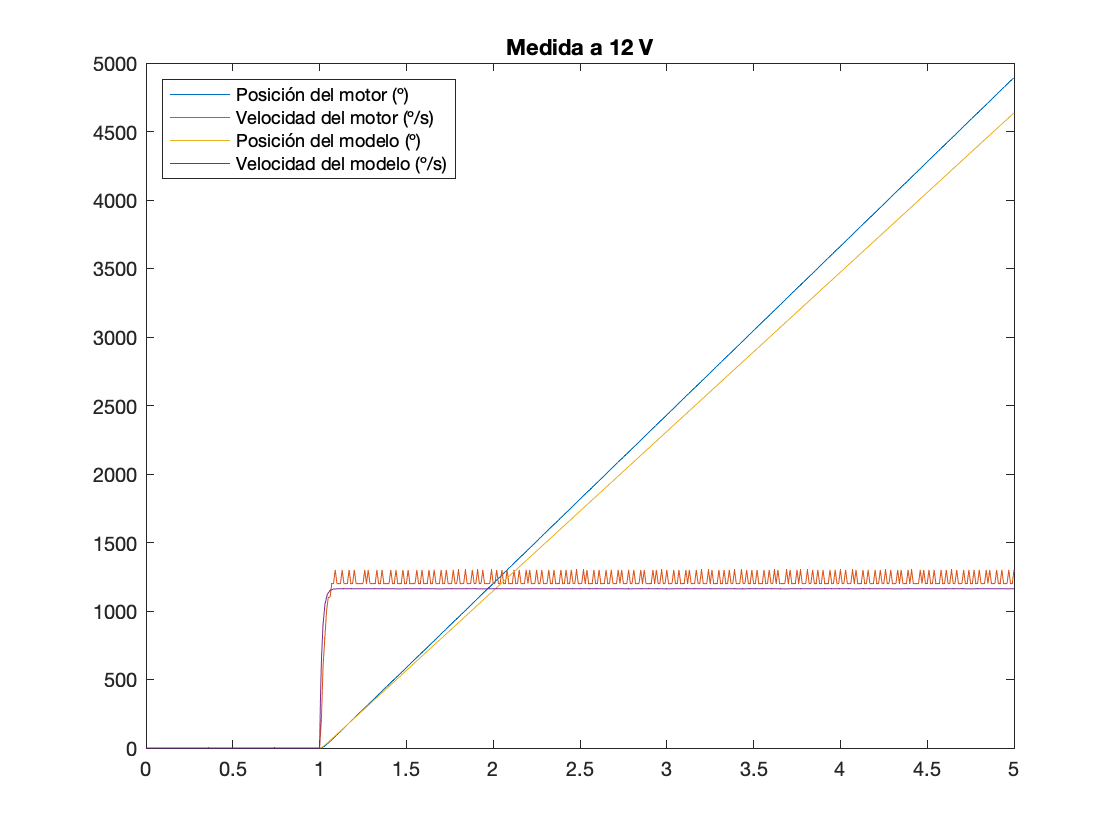
\includegraphics[height=8cm]{figs/p2/v12}
	\caption{Comparación a 12 V}  \label{comp12}
\end{figure}

\newpage
Como se puede apreciar en las figuras \ref{comp02}, \ref{comp06} y \ref{comp12}, la señal del modelo se aproxima bastante bien a los datos del motor. En el caso de los 2 V, se aprecia una mayor discrepancia, en parte por la resolución de la escala de posición y en parte porque el cociente de $k_e$ y $p$ obtenido para esta tensión es el menor y más distante del obtenido con los valores medios. Sin embargo, se puede concluir que el modelo se ajusta relativamente bien al motor, al menos para tiempos cortos de simulación. 

\section{Control del motor por realimentación de estados estimados}
Esta segunda sección se enfoca en la elaboración de un controlador para el motor en Simulink, partiendo de los modelos de motor realizados previamente. 
Para las simulaciones restantes se ha empleado otro modelo de motor ideal (equivalente salvo por una ganancia que tiene en cuenta la reductora del motor), estando su esquema presente en la figura \ref{ideal2}.

\begin{figure}[h!]
	\centering
	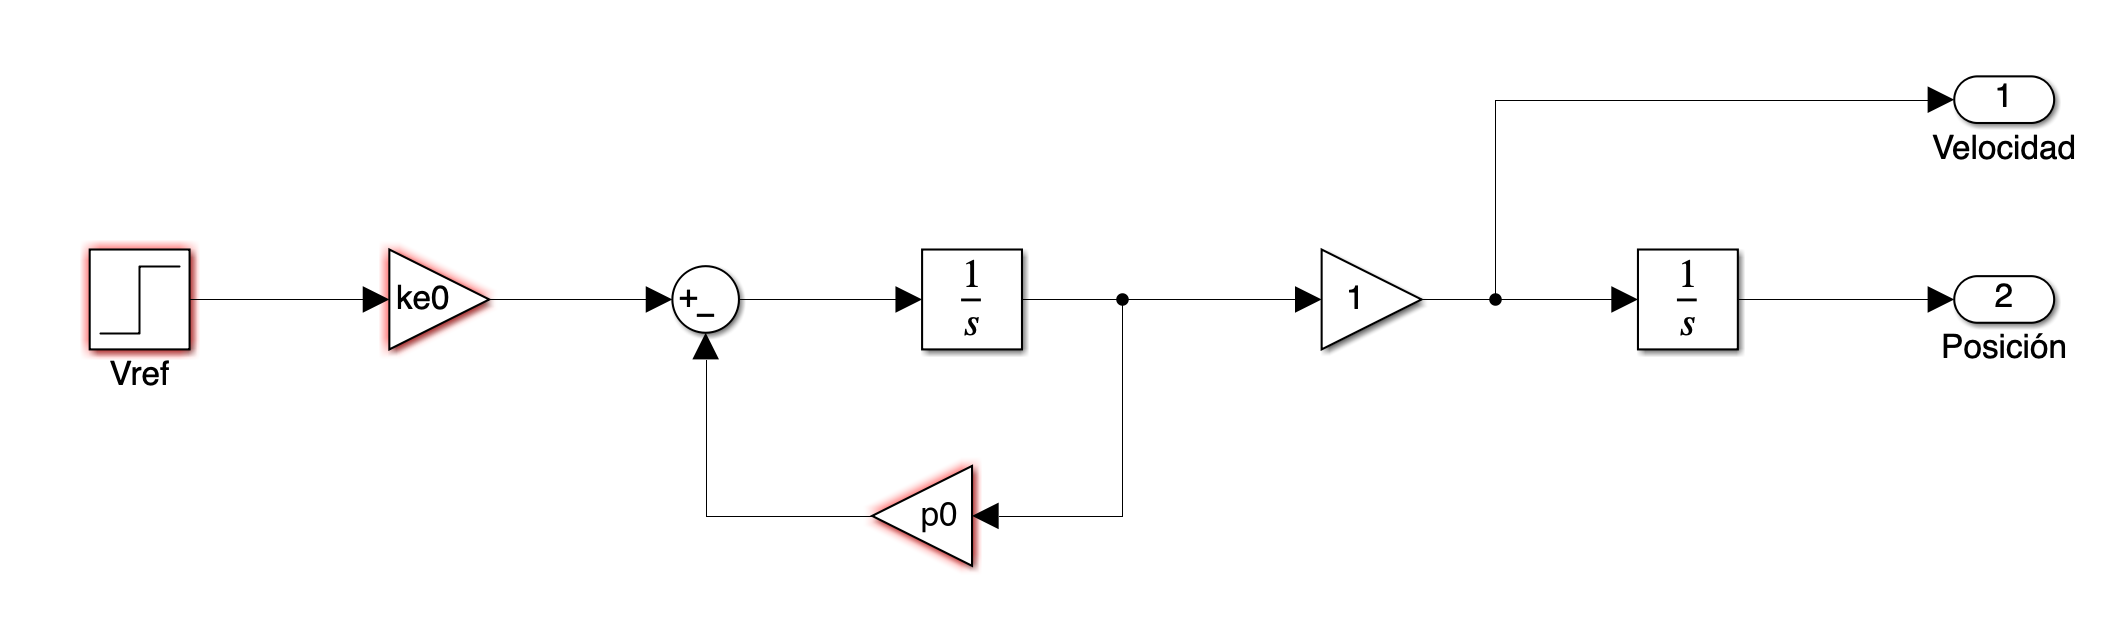
\includegraphics[height=4cm]{ideal2}
	\caption{Modelo de motor ideal considerando reductora} \label{ideal2}
\end{figure}
\subsection{Modelo completo del motor (Práctica 3)}
En primer lugar, se procede a construir un modelo más completo que el modelo de motor ideal elaborado al final de la sección anterior, que incluya también un modelo para simular los encoders y la alimentación con señales de PWM. 
Para la lectura de los encoders, se reutilizará el bloque de lectura empleado para el manejo en lazo abierto. \\

El sistema de alimentación tratará de simular las señales de PWM (Pulse-Width Modulation) que recibe el motor desde la placa. Entonces, se empieza por construir un bloque que genere una señal con las mismas características. \\

\begin{figure}[h!]
	\centering
	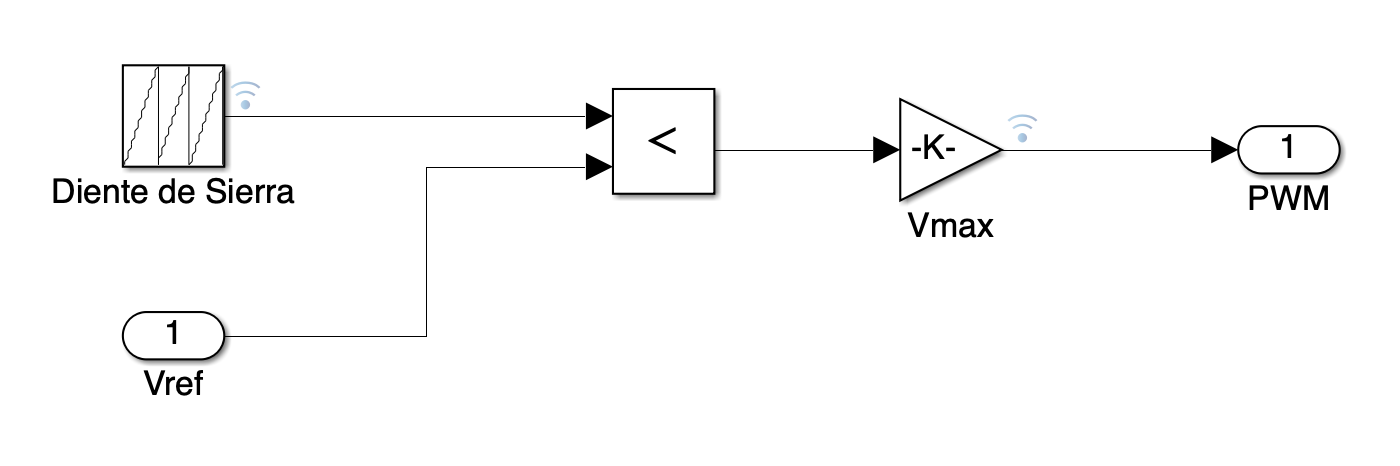
\includegraphics[height=4cm]{bloquepwm}
	\caption{Bloque de generación de señal de PWM}
\end{figure}


En el modelo final, este bloque se encontrará enmascarado y recibirá dos pará- metros: $T$, que dirigirá el periodo del diente de sierra y, en consecuencia, de la señal PWM (1ms) y $V_{max}$, indicador de la tensión máxima de esta señal (corresponderá con la tensión máxima nominal del motor, 12V).\\ 

El sistema de alimentación incluirá también un bloque en el que se ajuste $V_{ref}$, indicador de la tensión continua objetivo del bloque PWM (a menor $V_{ref}$, menor será el ciclo de trabajo de la señal PWM). Como el ciclo de trabajo se establece a través de una comparación de la tensión de la señal de diente de sierra. Para que el bloque PWM funcione correctamente, se ha de pasar una señal de $V_{ref}$ positiva. Si $V_{ref}$ es negativo, se multiplica por -1 la señal de PWM para que el motor avance en sentido contrario.\\
\begin{figure}[h!]
	\centering
	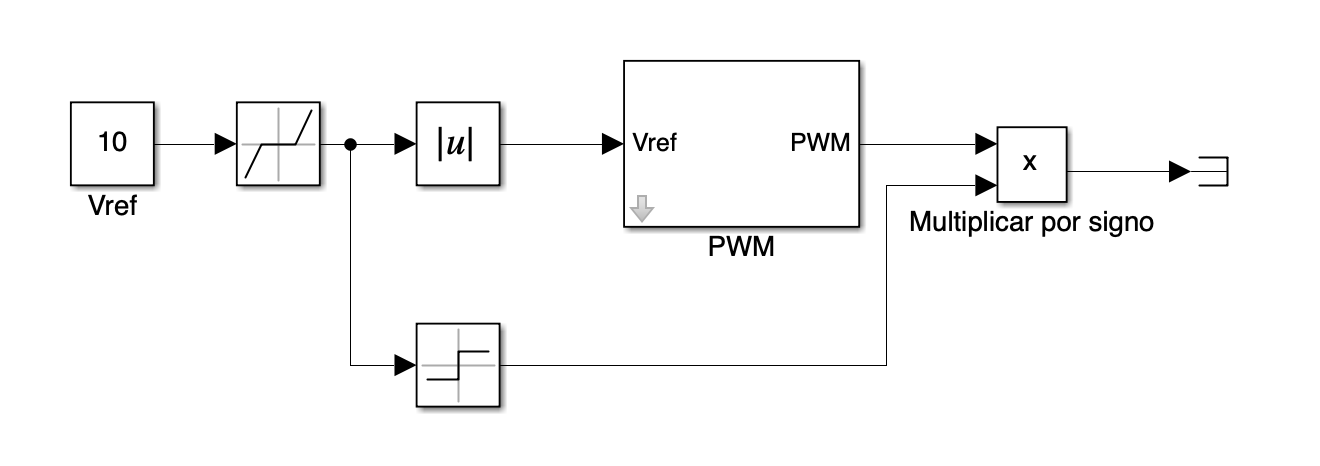
\includegraphics[height=4cm]{alimentador}
	\caption{Sistema de alimentación completo}
\end{figure}\\

A continuación se añade el modelo del motor ideal desarrollado previamente y se diseñan sus respectivos encoders para poder leer la posición y la velocidad. 
\begin{figure}[h!]
	\centering
	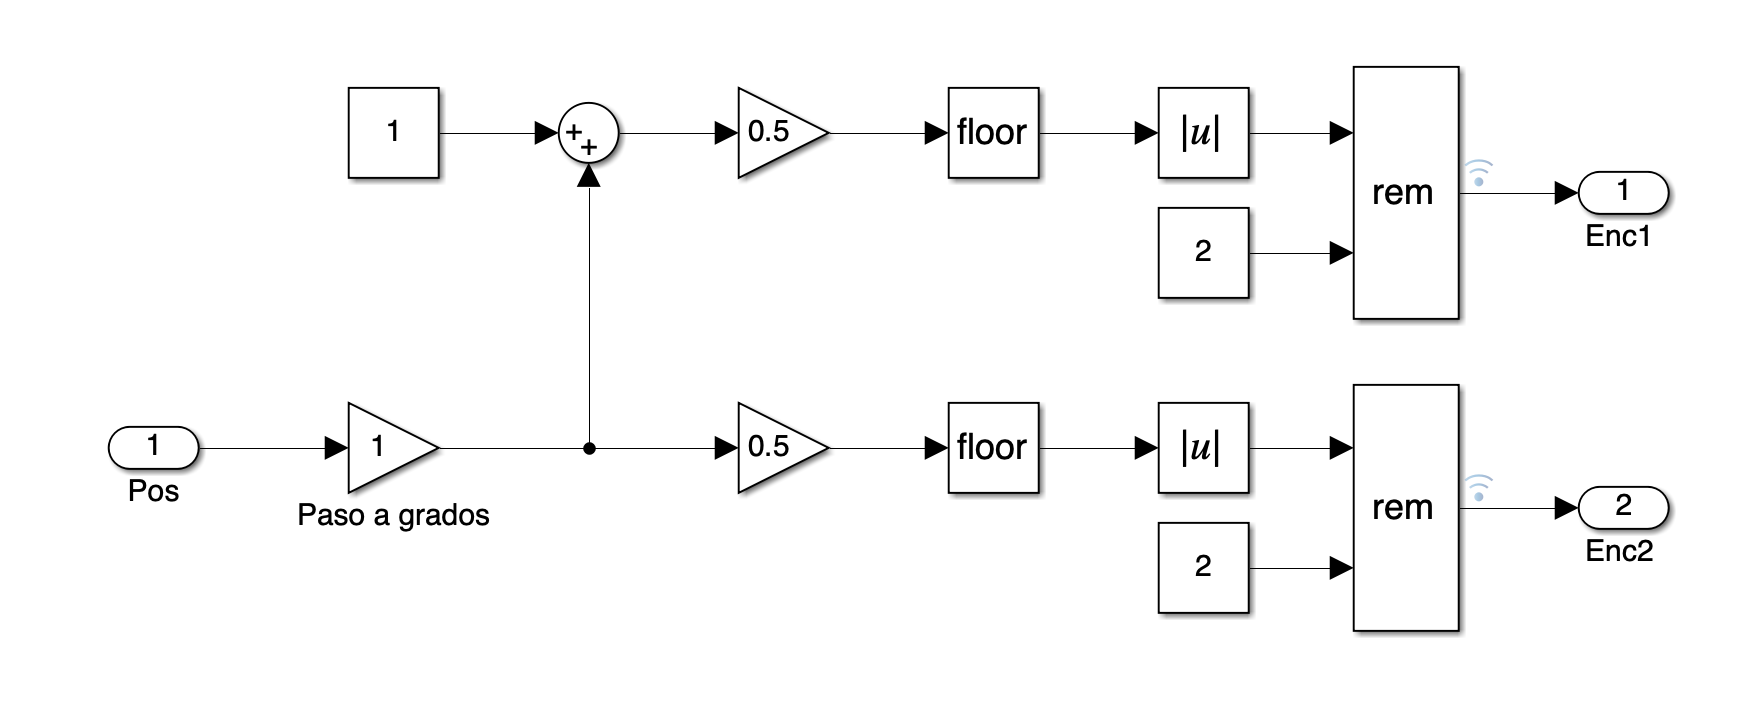
\includegraphics[height = 5cm]{encoders}
	\caption{Modelo de los encoders del motor}
\end{figure}

Por último, añadiendo el modelo reciclado para el lector de los encoders empleado en el lazo abierto, se termina de construir el modelo completo del motor real.  
\begin{figure}[h!]
	\centering
	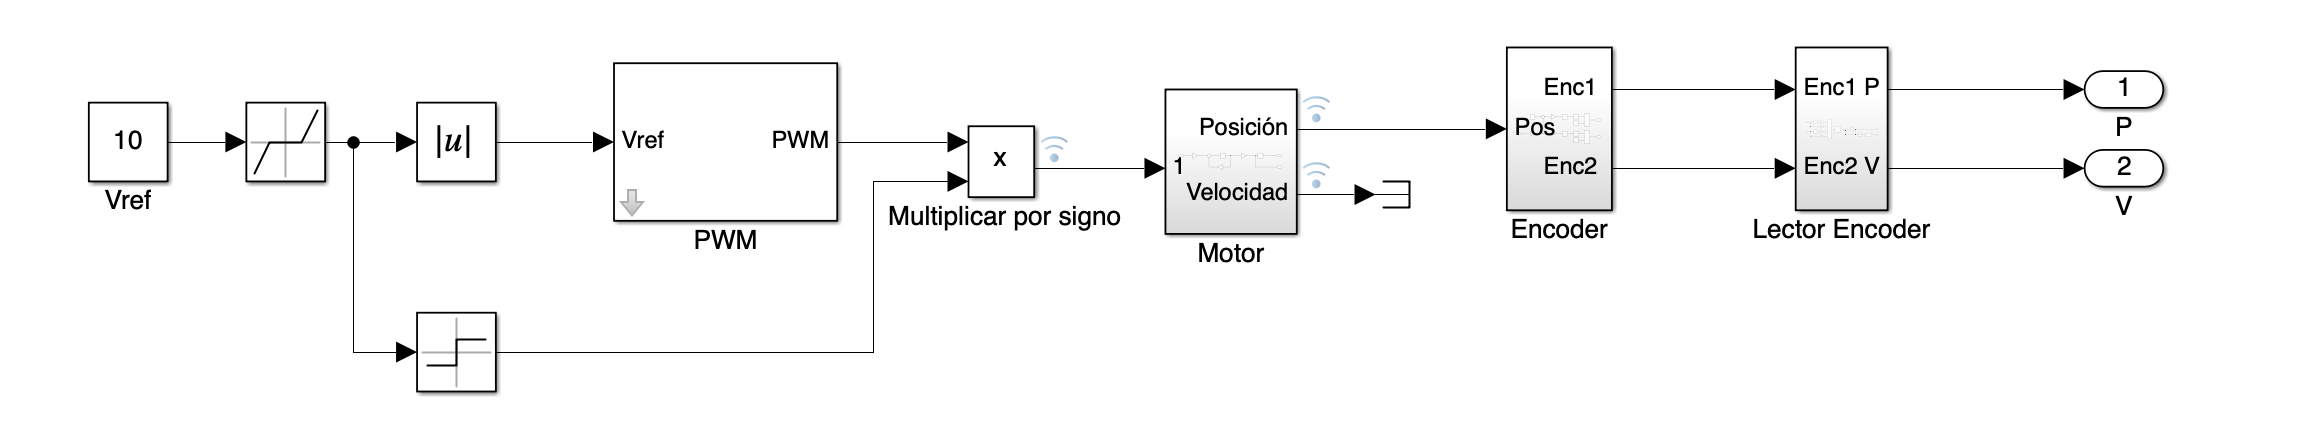
\includegraphics[height = 3cm]{real_completo}
	\caption{Modelo completo realista del motor}
\end{figure}
\subsubsection{Validez de los encoders}
A continuación se va a evaluar la validez de este sistema realista.
En primer lugar, se comparan las señales de los encoders con la señal directa del motor, es decir, la señal del motor ideal cuando recibe una tensión de PWM en vez de una tensión directa como en el modelo ideal. Las figuras \ref{encompleto02}, \ref{encompleto06} y \ref{encompleto12} muestran estas comparaciones para entradas de 2, 6 y 12 V otra vez.  \\
\begin{figure}[h!] 
	\centering
	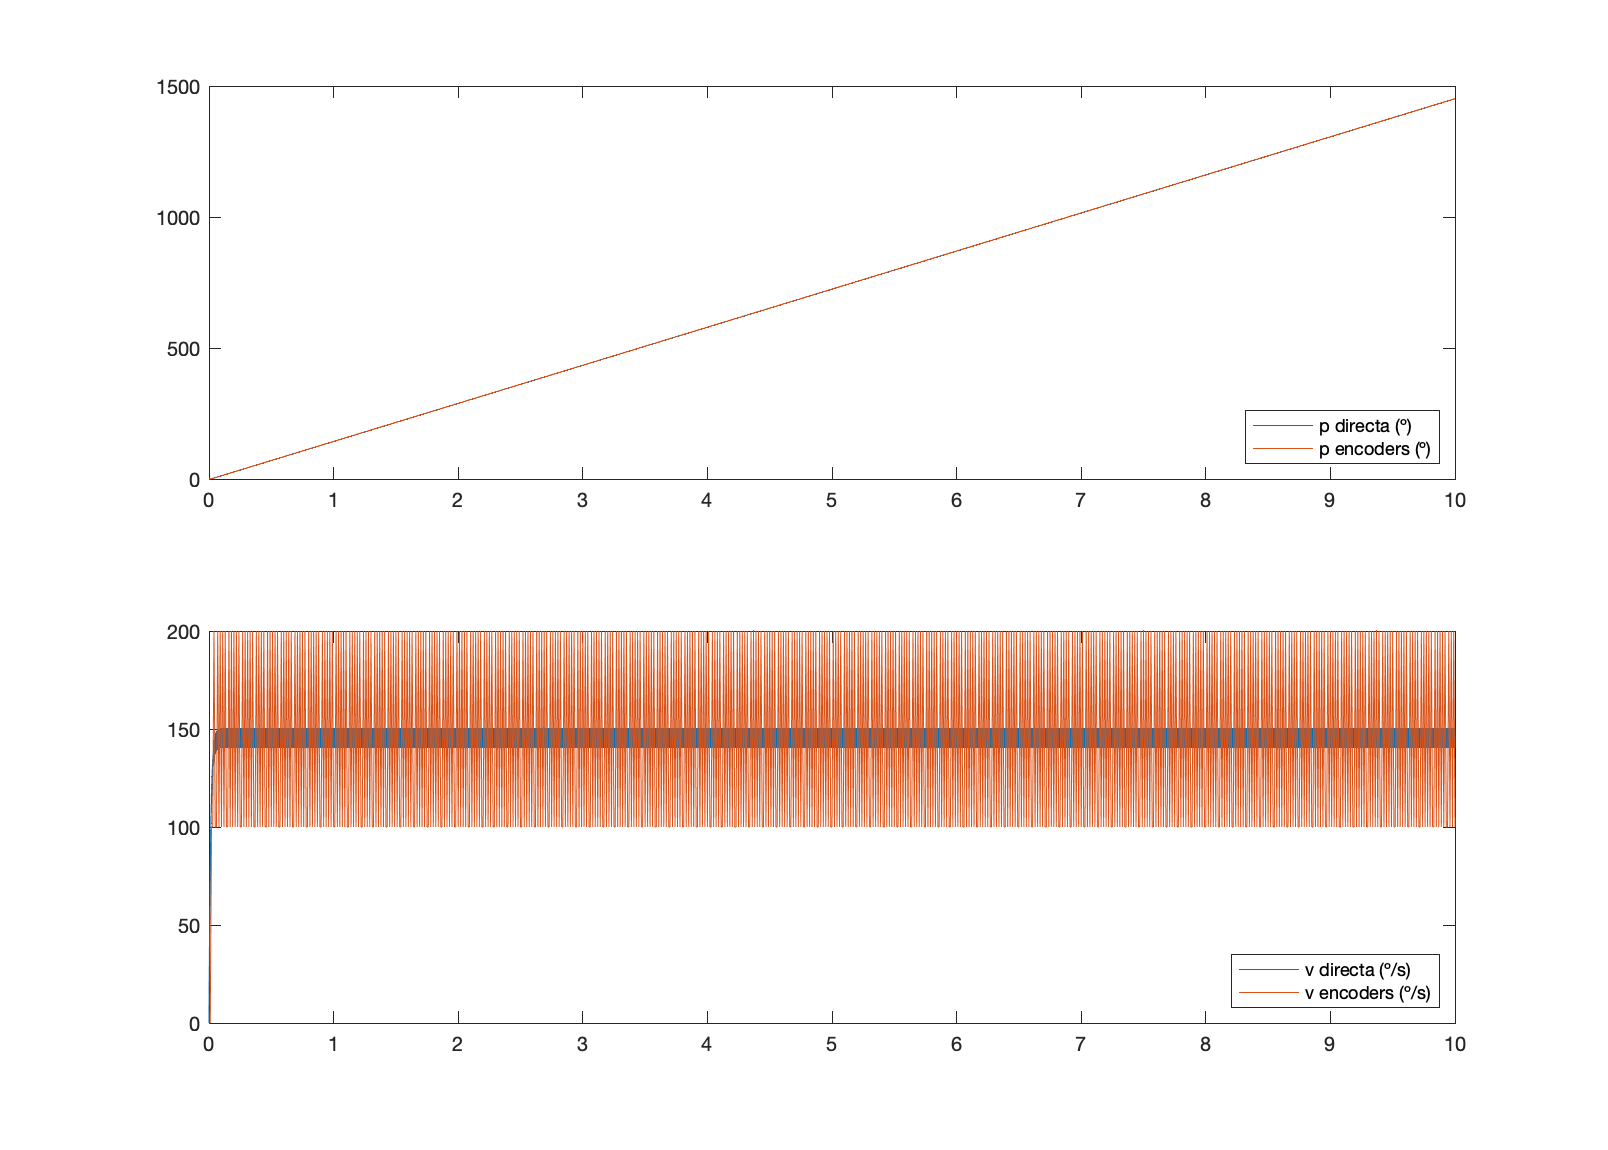
\includegraphics[height=7.5cm]{figs/p3/directaencoder2V} 
	\caption{Comparación modelo-encoders a 2V} \label{encompleto02}
\end{figure}
\begin{figure}[h!]
	\centering
	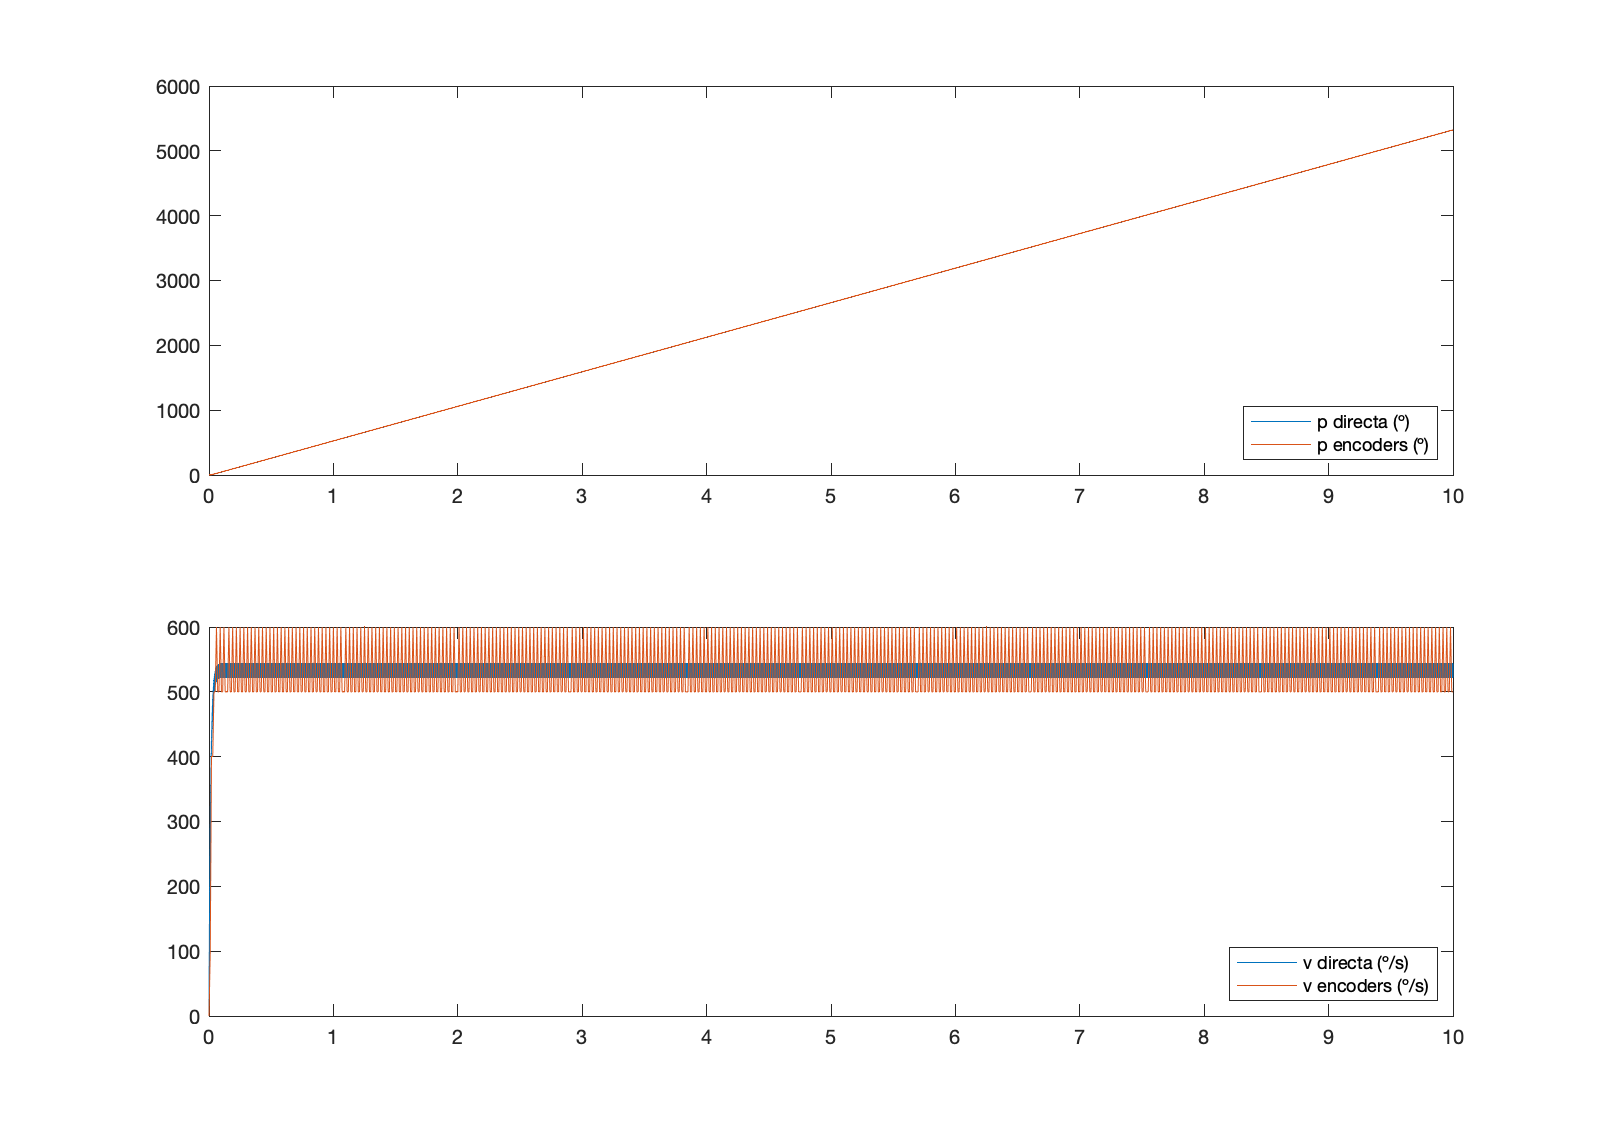
\includegraphics[height=7.5cm]{figs/p3/directaencoder6V} 
	\caption{Comparación modelo-encoders a 6V} \label{encompleto06}
\end{figure}
\begin{figure}[H]
	\centering
	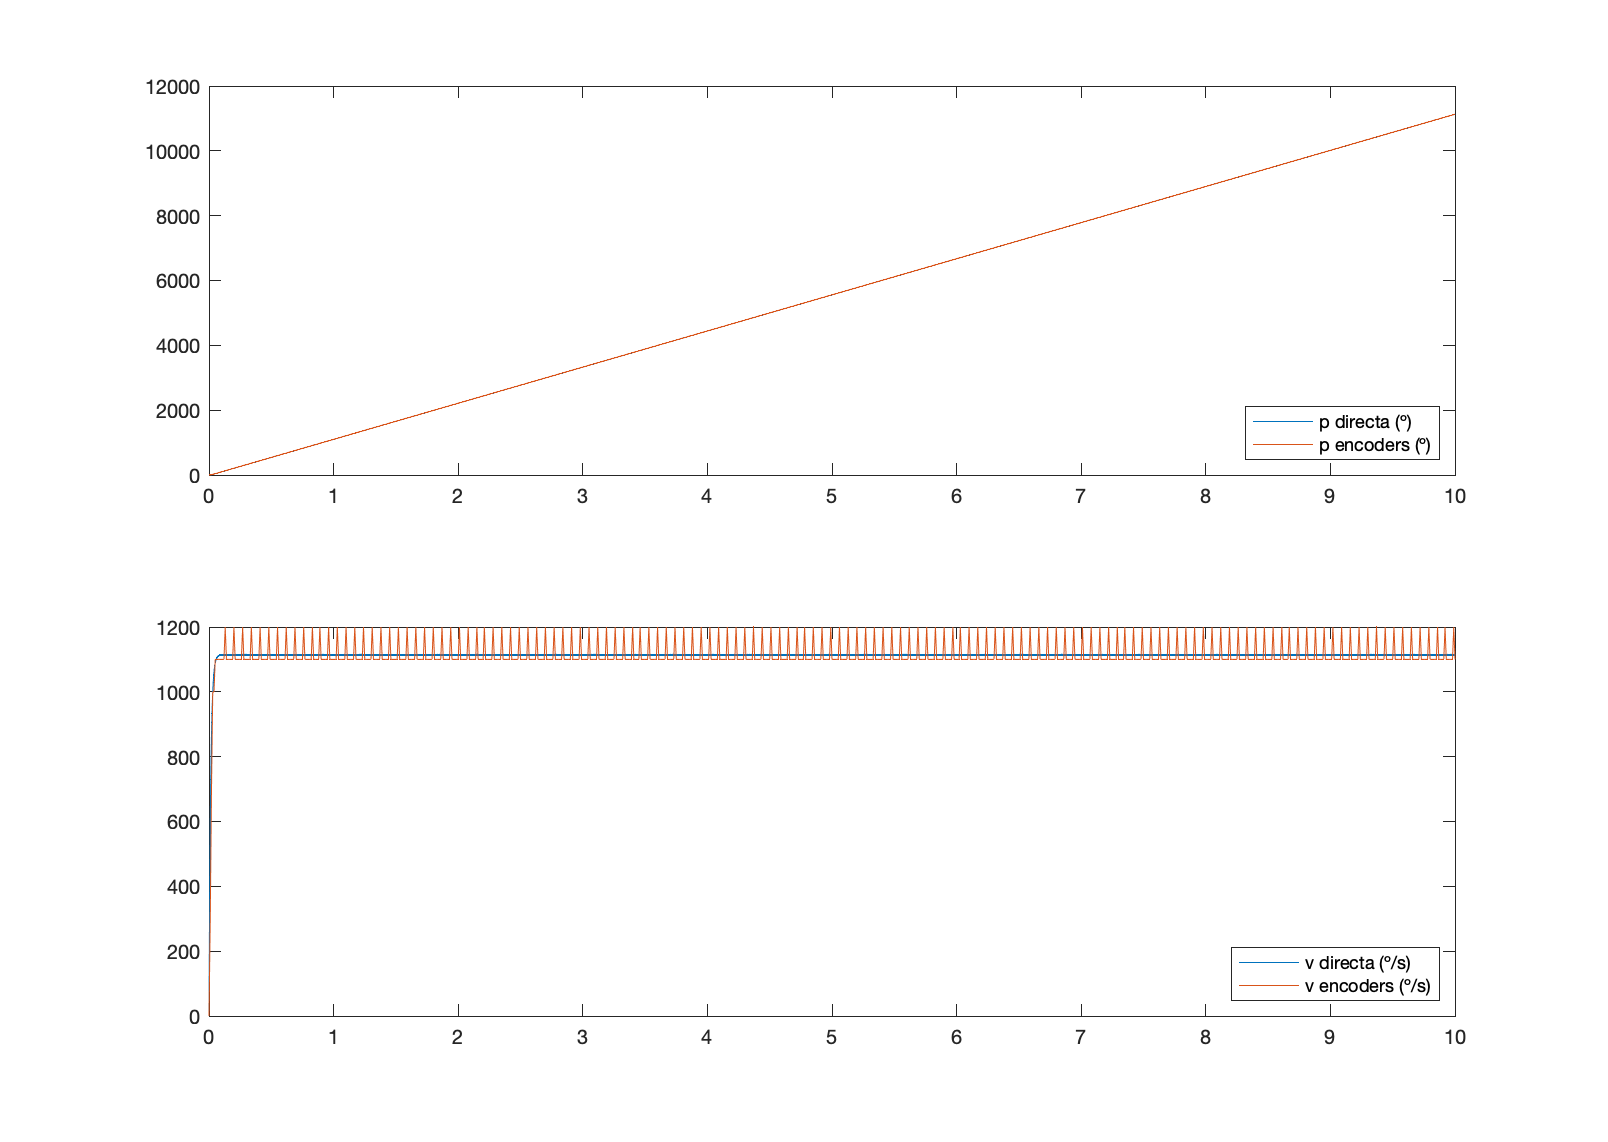
\includegraphics[height=7.5cm]{figs/p3/directaencoder12V}
	\caption{Comparación modelo-encoders a 12V}  \label{encompleto12}
\end{figure}

Como se puede apreciar en las figuras mencionadas, los estados leídos por los encoders son esencialmente iguales a las señales cargadas directamente desde la salida del motor ideal. 

\subsubsection{Comprobación de validez del modelo realista completo}
Ahora se repite el proceso de comprobación de validez del modelo con los datos reales del motor (figuras \ref{compreal02}, \ref{compreal06} y \ref{compreal12}).
\begin{figure}[H] 
	\centering
	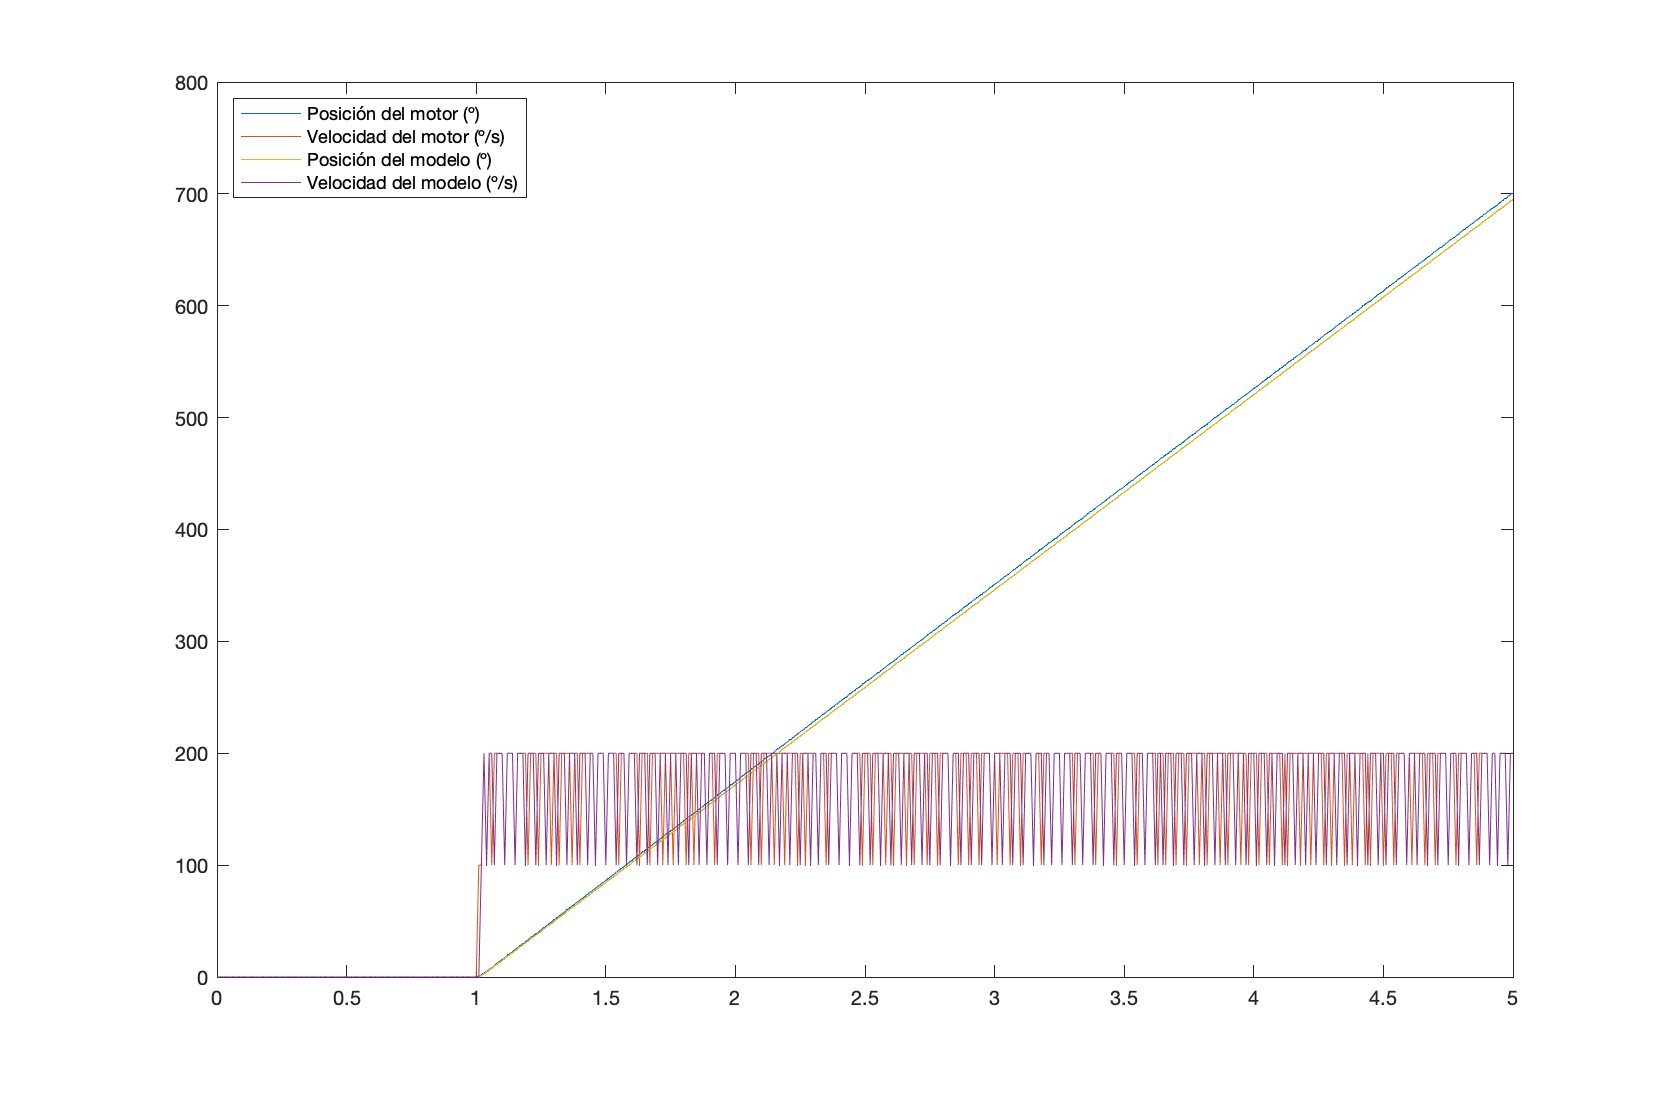
\includegraphics[height=8cm]{figs/p3/encodersmotormodelo2V} 
	\caption{Comparación motor-modelo a 2V} \label{compreal02}
\end{figure}
\begin{figure}[H]
	\centering
	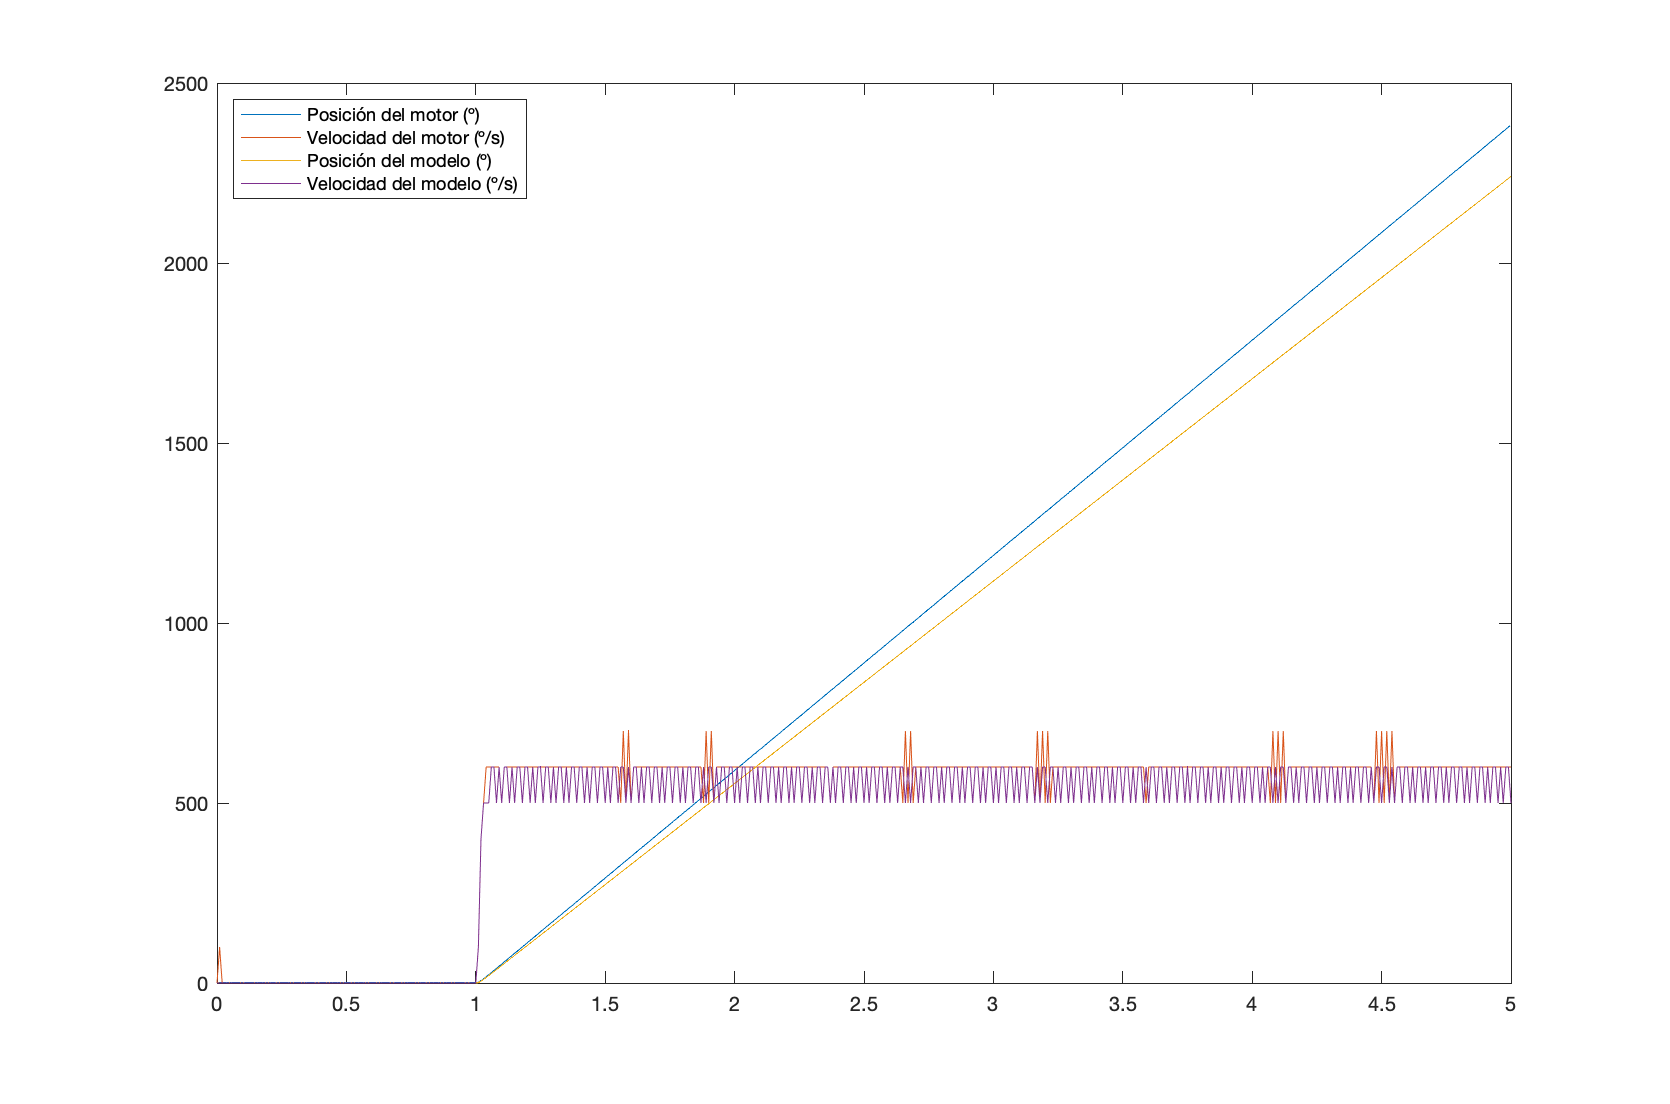
\includegraphics[height=8cm]{figs/p3/encodersmotormodelo6V} 
	\caption{Comparación motor-modelo a 6V} \label{compreal06}
\end{figure}
\begin{figure}[H]
	\centering
	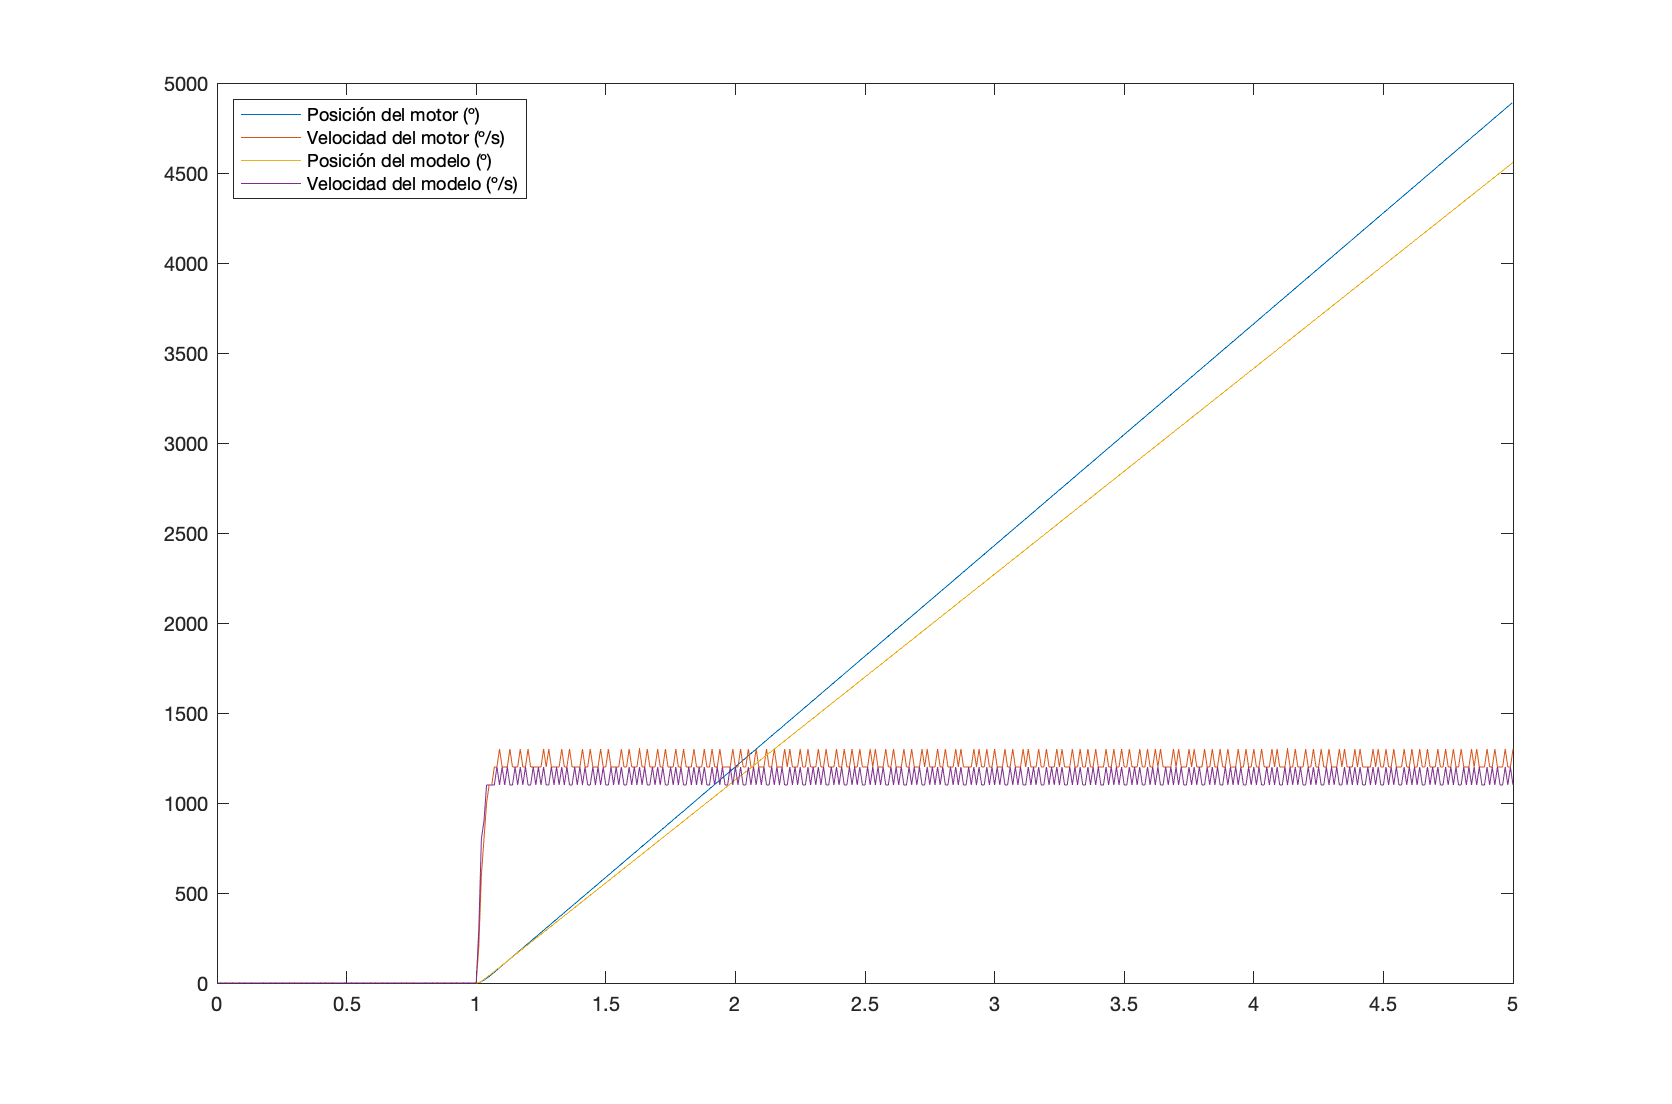
\includegraphics[height=8cm]{figs/p3/encodersmotormodelo12V}
	\caption{Comparación motor-modelo a 12V}  \label{compreal12}
\end{figure} 
Nótese que en estas simulaciones se aprecia cómo ahora las pendientes de las crectas del modelo han menguado (con respecto a las pendientes obtenidas para el motor ideal), y las velocidades del modelo se estabilizan alrededor de puntos ligeramente más bajos que para el modelo ideal. Esto puede ser consecuencia de la adición del bloque de zona muerta, que disminuye la entrada que llega al motor en 0.2 V. 

\subsection{Diseño de un controlador de la posición del motor por realimentación de estados estimados (Práctica 4)}
A continuación se tratará de diseñar un sistema que desplace el motor a una posición concreta a base de controlar su velocidad. Para esto se hará uso de un estimador que observe solamente la posición. Para empezar, se va a diseñar dicho control para el modelo ideal, por sencillez. \\

El sistema en cuestión vendrá descrito por las matrices
\begin{align}
		A &= \begin{bmatrix} 0 & 1 \\ 0 & -p \end{bmatrix}  \nonumber\\
		B &=  \begin{bmatrix} 0 \\ k_e \end{bmatrix}  \nonumber\\
		C &= \begin{bmatrix} 1 & 0 \end{bmatrix}  \nonumber\\
		D &= 0 \nonumber
\end{align}
tal que 
\begin{align}\label{sistema}
	\dot x(t) &= A x(t) + B u(t) \\
	y(t) &= Cx(t) + Du(t) \label{sistema2}
\end{align}
Y con la realimentación que se quiere llevar a cabo, 
\begin{equation}
	u(t) = -Kx(t) - Ly(t)
\end{equation}
Se calculan las ganancias del controlador $K$ y el observador $L$ en MatLab con el comando place. Para la ganancia de realimentación se han establecido unos polos de $-0.3p$ y $-0.4p$. 
Para el estimador, los polos se han dejado más negativos para asegurar que los estados estimados converjan a un estado real antes de que estos últimos se vayan a cero: $-1.2p$ y $-1.3p$.
Por último, se añade la acció integral, cuya ganancia se ha calculado con polos similares a los de la realimentación original, $-0.5p$, $-0.5p$ y $-0.7p$. Para esta última matriz se ha empleado el comando acker en vez de place, al haberse establecido un polo con multiplicidad 2. \\

La figura \ref{realimentado} muestra un esquema del modelo realimentado, incluyendo acción integral, acción directa y estimador.
\begin{figure}[H] 
	\centering
	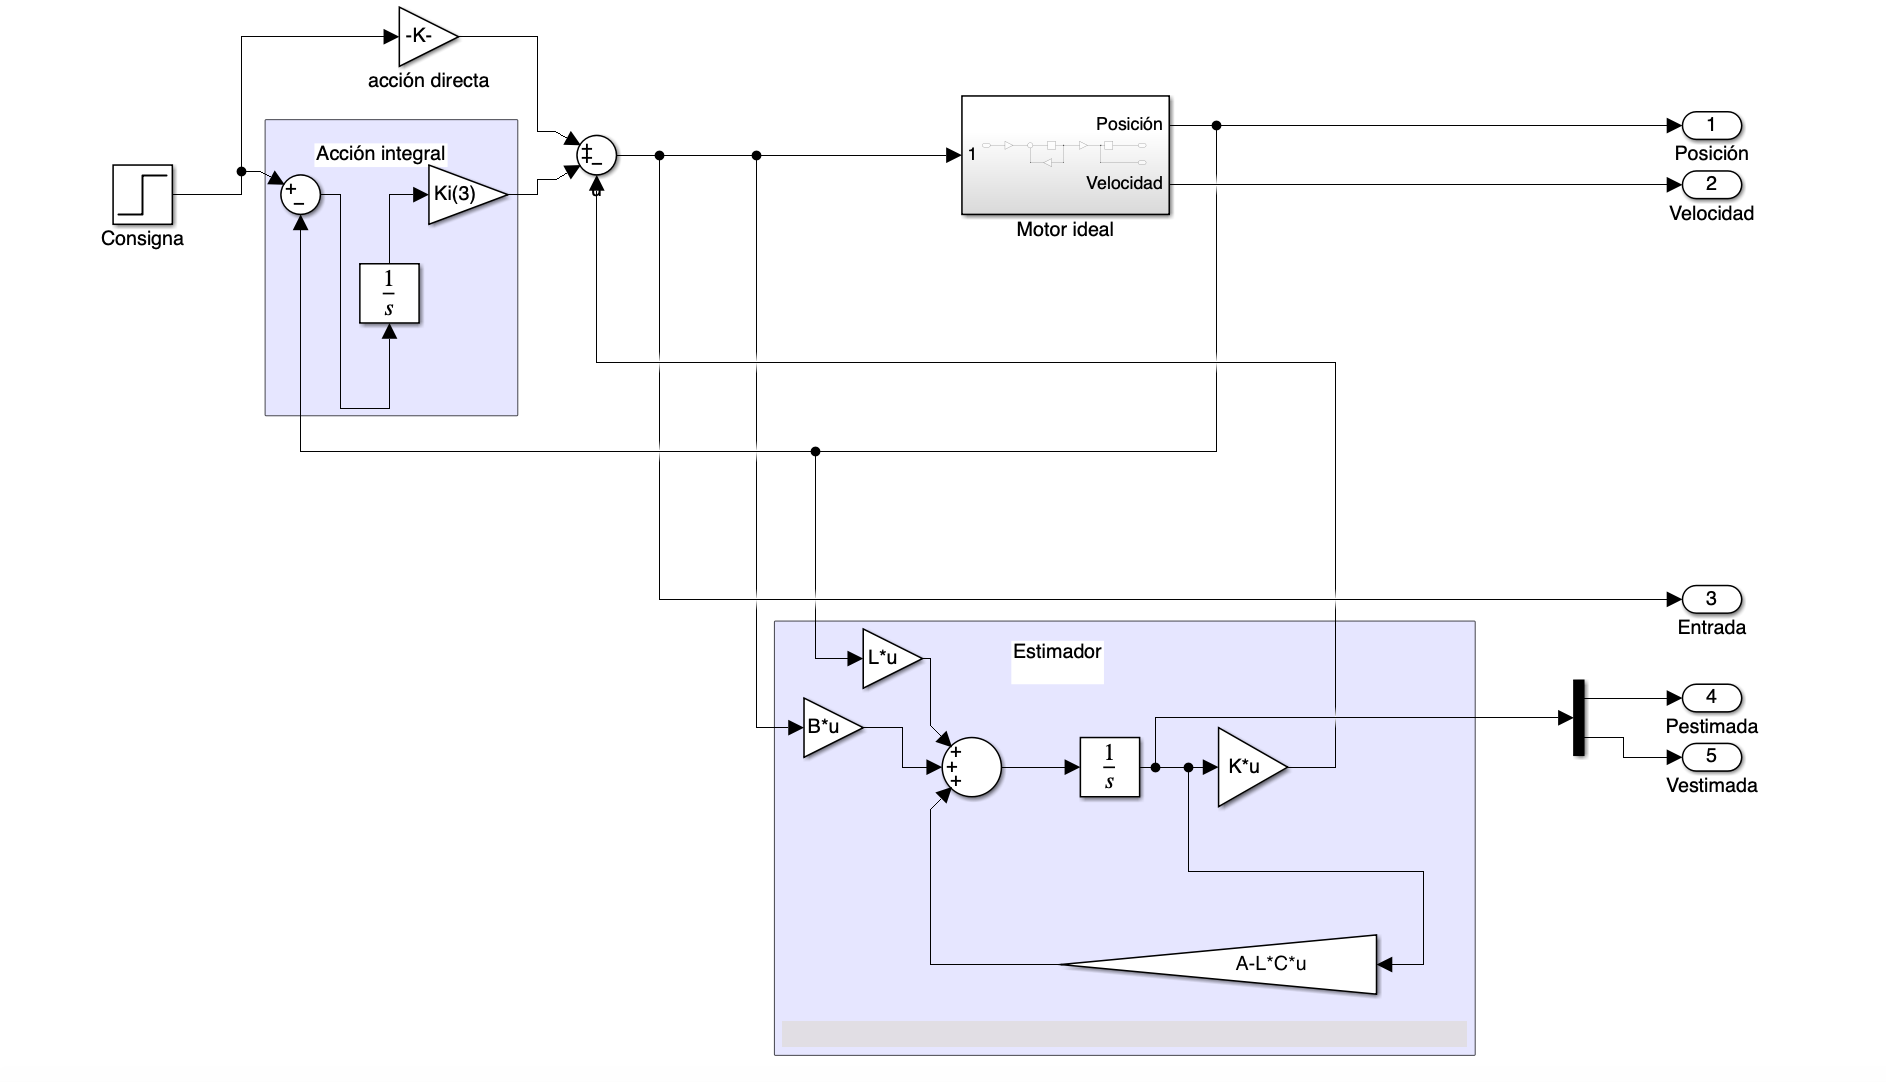
\includegraphics[height=8cm]{figs/p4/realimentado} 
	\caption{Modelo con control, acción directa y acción integral} \label{realimentado}
\end{figure}
\subsubsection{Estudio del efecto de los polos del sistema y del estimador}
En primer lugar, se realizan simulaciones del sistema (consigna de 90º, inicio del estimador a 10º, sin acción directa) para distintos valores de los polos de la realimentación así como de la acción integral.  \\

\begin{enumerate}
	\item 
	\begin{itemize}
		\item Polos del sistema: $-0.5p, -0.5p, -0.7p$
		\item Polos del estimador: $-1.2p, -1.3p$
	\end{itemize}

\begin{figure}[H]
	\centering
	\includegraphics*[height = 7.5cm]{figs/p4/ki05}
	\caption{Simulación del sistema realimentado}
\end{figure}
A primera vista se ve que el sistema se comporta adecuadamente: la posición converge rápidamente a la consigna, y la velocidad y la realimentación se van a 0. Sin embargo, la señal de entrada máxima supera por algo menos de un voltio el voltaje máximo que puede recibir el motor real, por lo que estos polos no son óptimos. 
\item 
	\begin{itemize}
		\item Polos del sistema: $-0.05p, -0.05p, -0.07p$
		\item Polos del estimador: $-1.2p, -1.3p$
	\end{itemize}


\begin{figure}[H]
	\centering
	\includegraphics*[height = 7.5cm]{figs/p4/ki005}
	\caption{Simulación con polos más pequeños}
\end{figure}

Se aprecia que el sistema tarda ahora mucho más en converger, pero la señal de entrada es mucho menor, su máximo estando lejos de la tensión de saturación. \\

\item 
	\begin{itemize}
		\item Polos del sistema: $-5p, -5p, -7p$
		\item Polos del estimador: $-1.2p, -1.3p$
	\end{itemize}

	\begin{figure}[H]
		\centering
		\includegraphics*[height = 7.5cm]{figs/p4/ki5}
		\caption{Simulación con polos más grandes}
	\end{figure}
		

Ahora el sistema converge a la consigna muy velozmente, pero la señal de entrada supera por órdenes de magnitud los 12 V máximos que puede suministrar el sitema antes de saturar, luego es una solución poco reocmendable.
\end{enumerate}

Ahora uno puede estudiar qué ocurre al modificar los polos del estimador.

\begin{enumerate}
\item 
	\begin{itemize}
		\item Polos del sistema: $-0.5p, -0.5p, -0.7p$
		\item Polos del estimador: $-0.12p, -0.13p$
	\end{itemize}


\begin{figure}[H]
	\centering
	\includegraphics*[height = 7.5cm]{figs/p4/l011}
	\caption{Simulación con polos más pequeños para el estimador} \label{slo}
\end{figure}
La figura \ref{slo} muestra unos resultados poco interesantes, puesto que lo único apreciable es una mayor tiempo para que el estimador converja a los estados del sistema, pero la señal de realimentación tiene la misma forma, es decir, no se consigue bajar el máximo de tensión de entrada a valores permitidos.  
\item 
	\begin{itemize}
		\item Polos del sistema: $-0.5p, -0.5p, -0.7p$
		\item Polos del estimador: $-12p, -13p$
	\end{itemize}

	\begin{figure}[H]
		\centering
		\includegraphics*[height = 7.5cm]{figs/p4/l11}
	
		\caption{Simulación con polos más grandes para el estimador} \label{fas}
	\end{figure}
		

\end{enumerate}
Se confirma por lo general que, cuanto más negativos sean los polos del estimador, los estados estimados convergen más rápido a los estados de sistema. En el caso de \ref{fas}, el efecto combinado de la rápida convergencia del estimador a los estados del modelo con la posición inicial incorrecta del estimador induce un pico de tensión en la señal de entrada al comienzo de la simulación. 

\subsubsection{Efecto de la acción directa}
Ahora se estudia la acción directa. Esto fuerza una señal constante para el modelo. Al haber control integral implicada en el modelo, su único efecto será el modificar la posición inicial de la entrada u. 

\begin{figure}[H]
	\centering
	\includegraphics*[height = 7.5cm]{figs/p4/ad10}

	\caption{Simulación con ganancia de 10 para la acción directa}
\end{figure}

Como se puede apreciar, el sistema se comporta de manera muy similar, habiendo solo variado la posición a t = 0 de la señal de entrada. 

\subsubsection{Influencia del error en la posición inicial}
Por último, se observa el efecto de modificar la posición inicial del estimador en la evolución general del mismo y consecuentes repercusiones en el sistema. 
\begin{figure}[H]
	\centering
	\includegraphics*[height = 7.5cm]{figs/p4/ini0}
	\caption{Simulación con posición inicial en el origen}
\end{figure}
\begin{figure}[H]
	\centering
	\includegraphics*[height = 7.5cm]{figs/p4/ini-100}
	\caption{Simulación con posición inicial de -100º}
\end{figure}

En este caso, si bien no se aprecia una notable mejoría de los tiempos de convergencia del sistema, cabe destacar la diferencia de tiempo que tarda en converger el estimador si empieza más cerca de la posición correcta del sistema, y la menor señal de realimentación al principio de la simulación. 

\subsection{Discretización del modelo (Práctica 5)}
Hasta ahora el control se ha desarrollado para un sistema con entradas y salidas continuas, como es el caso del modelo ideal del motor. Ahora se extenderán los sistemas de control desarrollados al modelo realista del motor y posteriormente se aplicarán al motor original. \\

Las señales de estos dos últimos sistemas son señales discretas, lo que implica que hay que modificar el control para que funcione también para señales discretas. 
Ahora el sistema, en vez de ser dependiente de valores de tiempo, como antes, pasará a funcionar basado en una nueva variable entera $n$, tal que $t = nT$, siendo $T$ el tiempo de muestreo del sistema (ajustado a 0.1 ms). 
El sistema ahora vendrá descrito por cuatro matrices nuevas: $F$, $G$, $C$ y $D$, tales que
\begin{align} \label{zistema}
	x(n + 1) &= Fx(n) + Gu(n) \\
	y(n) &= Cx(n) + Du(n).
\end{align}
\newpage
Esto es un sistema análogo al descrito por las expresiones \ref{sistema} y \ref{sistema2}, pero con otro dominio discreto. 
Las matrices nuevas se calculan con MatLab a partir de las del modelo de dominio continuo, definiendo primero un sistema con las matrices $A$, $B$, $C$ y $D$ con el comando ss y posteriormente discretizándolo con el comando c2d. Nótese que ahora, para que el control funcione, hay que discretizar también los polos con los que se van a calcular las ganancias de la realimentación. 
Teniendo en cuenta las respuestas producidas por los polos del modelo continuo, 
\begin{equation}
	y(t) \sim e^{\lambda_i t} \rightarrow y(nT) \sim e^{\lambda_i nT} = (e^{\lambda_i T})^n
\end{equation}
se ve que se puede aplicar la transformación 
\begin{equation}
	\Lambda_i = e^{\lambda_iT},
\end{equation}
donde $\Lambda_i$ es un polo arbitrario del sistema nuevo calculado a partir de uno de los polos del sistema continuo ($\lambda_i$). Esta transformación se aplicará para obtener los polos con los que se calcularán las ganancias de realimentación, observación de estados y acción integral discretas. \\

El modelo de simulink del sistema discreto es muy similar al del sistema continuo, con la excepción de que ahora en vez de integradores se hace uso de bloques \textit{Unit Delay} y las señales cuentan con \textit{Zero-order Hold}s.
\begin{figure}[H]
	\centering
	\includegraphics*[height = 7cm]{figs/p5/discreto}
	\caption{Modelo del sistema con control discreto}
\end{figure}
\subsubsection{Influencia de la posición de los polos}
De nuevo se procede a estudiar cómo afecta la elección de polos a la evolución del sistema. Se simula para una consigna de 100º esta vez, iniciando el estimador en el origen y sin acción directa. 
\begin{enumerate}
	\item 
	\begin{itemize}
		\item Polos del sistema: $e^{-0.5pT}, e^{-0.5pT}, e^{-0.7pT}$
		\item Polos del estimador: $e^{-1.2pT}, e^{-1.2pT}$
	\end{itemize}

\begin{figure}[H]
	\centering
	\includegraphics*[height = 7.5cm]{figs/p5/ki05}
	\caption{Simulación del sistema discretizado}
\end{figure}
\item 
	\begin{itemize}
		\item Polos del sistema: $e^{-0.05pT}, e^{-0.05pT}, e^{-0.07pT}$
		\item Polos del estimador: $e^{-1.2pT}, e^{-1.2pT}$
	\end{itemize}

\begin{figure}[H]
	\centering
	\includegraphics*[height = 7.5cm]{figs/p5/ki005}
	\caption{Simulación con polos más pequeños}
\end{figure}

\item 
	\begin{itemize}
		\item Polos del sistema: $e^{-5pT}, e^{-5pT}, e^{-7pT}$
		\item Polos del estimador: $e^{-1.2pT}, e^{-1.2pT}$
	\end{itemize}

\begin{figure}[H]
	\centering
	\includegraphics*[height = 7.5cm]{figs/p5/ki5}
	\caption{Simulación con polos más grandes}
\end{figure}

\end{enumerate}
En general, el sistema se comporta de manera similar que en el caso ideal. Al simular con polos más negativos, el sistema evoluciona mucho más rápido de lo que el estimador converge a los estados reales, por lo que se aprecia una señal oscilante hasta que al final se estabiliza.

\begin{enumerate}
	\item 
		\begin{itemize}
			\item Polos del sistema: $e^{-0.5pT}, e^{-0.5pT}, e^{-0.7pT}$
			\item Polos del estimador: $e^{-0.12pT}, e^{-0.12pT}$
		\end{itemize}
	
	
	\begin{figure}[H]
		\centering
		\includegraphics*[height = 7.5cm]{figs/p5/l011}
		\caption{Simulación con polos más pequeños para el estimador} \label{slo2}
	\end{figure}
	La figura \ref{slo2} indica que en este caso, los valores de los polos del estimador son tan pequeños que el sistema se estabiliza en la consigna mucho antes de que converja a los estados reales, por lo que se aprecia diferencia entre los resultados de las estimaciones y las salidas del modelo del motor al final de la simulación.
	\item 
		\begin{itemize}
			\item Polos del sistema: $e^{-0.5pT}, e^{-0.5pT}, e^{-0.7pT}$
			\item Polos del estimador: $e^{-12pT}, e^{-12pT}$
		\end{itemize}
	
		\begin{figure}[H]
			\centering
			\includegraphics*[height = 7.5cm]{figs/p5/l11}
		
			\caption{Simulación con polos más grandes para el estimador} 
		\end{figure}
			
	
	\end{enumerate}

\subsubsection{Efecto de la acción directa}
De nuevo, se puede ajustar una ganancia $f$ arbitraria para la acción directa, que altere los resultados iniciales de la simulación pero no gravemente la convergencia. 
\begin{figure}[H]
	\centering
	\includegraphics*[height = 7.5cm]{figs/p4/ad10}

	\caption{Simulación con ganancia de 1 para la acción directa}
\end{figure}
\subsubsection{Efecto de la acción integral}
Por último, hasta ahora solo se han hecho simulaciones en las que interviene el control integral. De modo que se observará el sistema con las mismas condiciones iniciales mencionadas al comienzo de esta sección, pero descartando la acción integral. En este caso, se hará uso de la acción directa para que el sistema alcance la posición de consigna, por lo que ya no es arbitraria.
Se puede calcular la ganancia $f$ necesaria para que el sistema alcance el estado estacionario correcto como:
\begin{equation}
	f = \left[C[\mathbb{I} - (F - GK^{-1})]^{-1} G \right]^{-1} 
\end{equation}
que, al sustituir las matrices del sistema discreto, resulta $f \approx 0.73$.
\begin{figure}[H]
	\centering
	\includegraphics*[height = 7.5cm]{figs/p5/noai}

	\caption{Simulación con $f$ ajustada y sin acción integral} 
\end{figure}
Se puede comprobar que el sistema igualmente se estabiliza en la posición de consigna de 100º. 
\subsection{Controlador discreto completo y aplicación al motor real (Práctica 6)}
A continuación, se va a incluir un sistema que prevenga los problemas de \textit{wind-up}. Si se tiene en cuenta la saturación del motor a 12 V, la acción integral puede inducir oscilaciones en el sistema que lo desestabilicen. Esto se puede prevenir disminuyendo (o eliminando) la acción integral mientras se está en estado de saturación, de manera que el error integral no se desestabilice. 
\begin{figure}[H] 
	\centering
	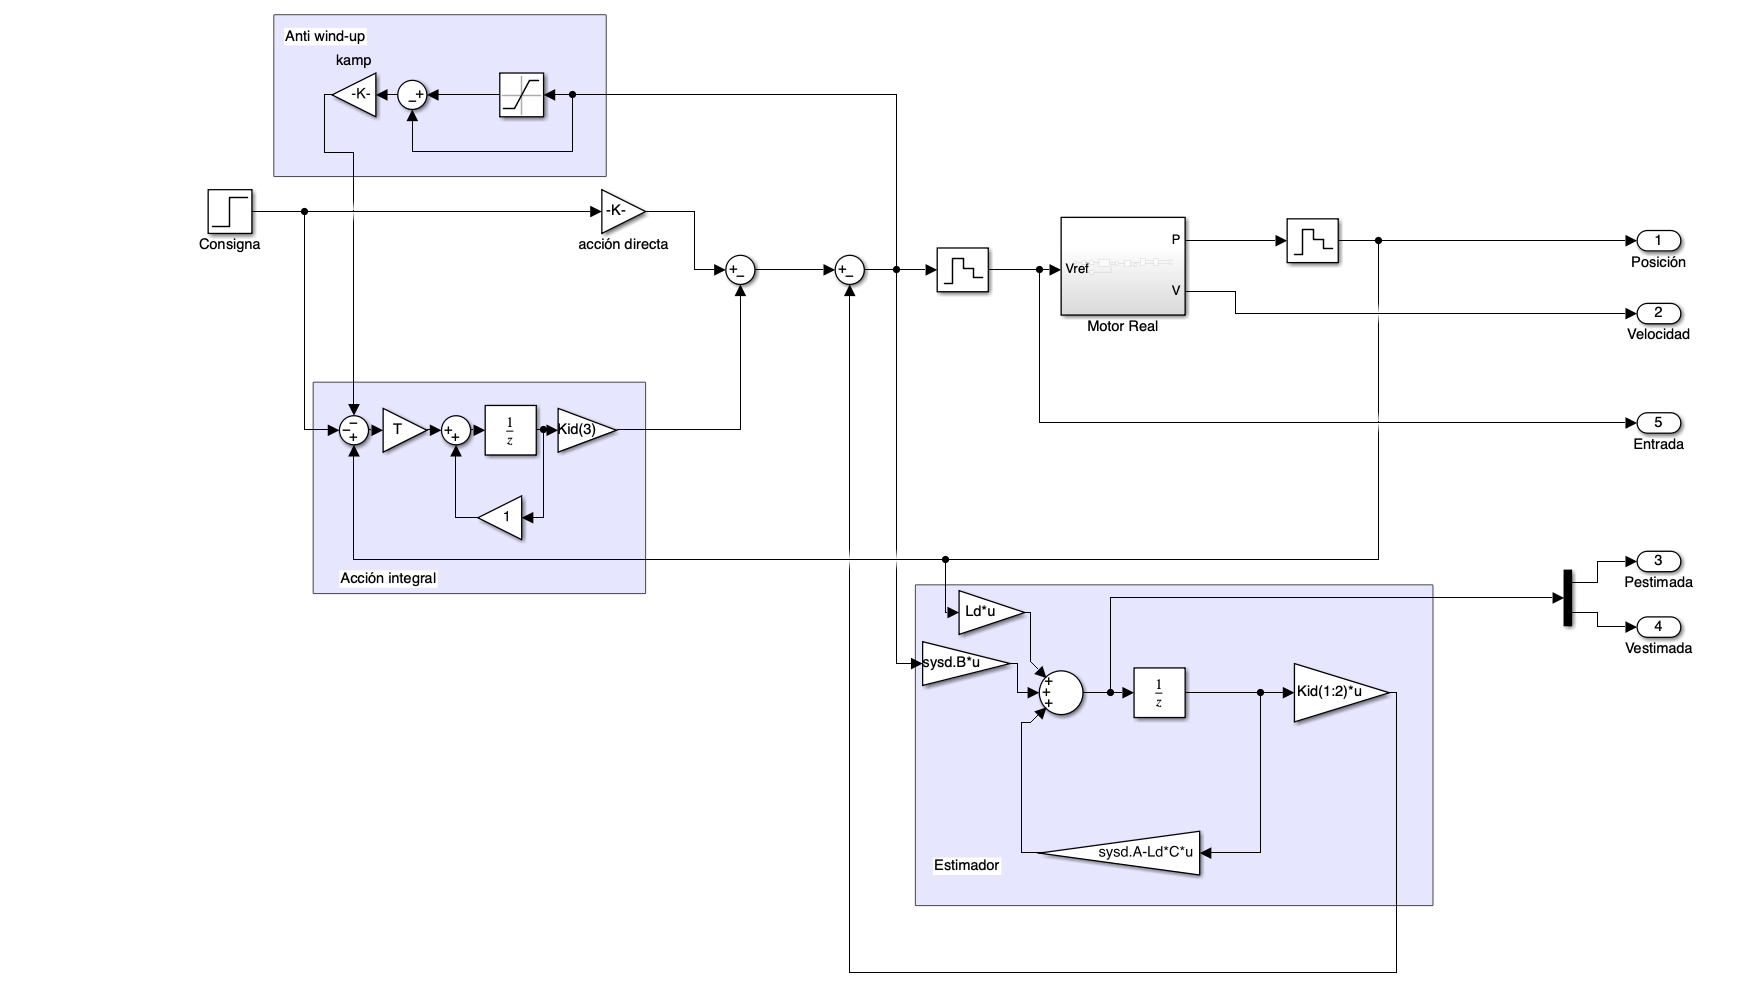
\includegraphics[height=8cm]{figs/p6/antiwup} 
	\caption{Modelo discreto con anti-windup} \label{antiwup}
\end{figure}


\subsubsection{Efecto del \textit{anti-windup}}
Recuperando la simulación para polos del sistema  $\Lambda_{1, 2} = e^{-5pT}, \Lambda_i = e^{-7pT}$, que presentaba oscilaciones, se puede comprobar fácilmente el efecto del \textit{anti-windup}.
\begin{figure}[H]
	\centering
	\includegraphics*[height = 7.5cm]{figs/p6/kamp0}
	\caption{Simulación para $k_{amp} = 0$ (sin \textit{anti-windup})}
\end{figure}
\begin{figure}[H]
	\centering
	\includegraphics*[height = 7.5cm]{figs/p6/kamp05}
	\caption{Simulación para $k_{amp} = 0.5$}
\end{figure}
\begin{figure}[H]
	\centering
	\includegraphics*[height = 7.5cm]{figs/p6/kamp05}
	\caption{Simulación para $k_{amp} = 1$}
\end{figure}

Como se puede observar, el efecto del \textit{anti-windup} amortigua drásticamente las oscilaciones para estas condiciones de simulación, aunque no hay una diferencia notable para los distintos valores no nulos de la ganancia $k_{amp}$.

\subsubsection{Aplicación del controlador al motor real}
Por último, solo queda comprobar que este modelo de controlador por realimentación de estados funciona para el dispositivo real. Se reemplaza el modelo realista por el motor real, con cuidado de pasarle por separado el signo de la señal de entrada y el valor absoluto de la señal normalizada sobre el voltaje máximo. 
\begin{figure}[H]
	\centering
	\includegraphics*[height = 7.5cm]{figs/p6/kamp05}
	\caption{Simulación para $k_{amp} = 0.5$}
\end{figure}
\begin{figure}[H]
	\centering
	\includegraphics*[height = 7.5cm]{figs/p6/cons180} 
	\caption{Simulación para posición de consigna de 180º} \label{poscos}
\end{figure}
\begin{figure}[H]
	\centering
	\includegraphics*[height = 8cm]{figs/p6/cons-240}
	\caption{Simulación para posición de consigna de -240º} \label{negcos}
\end{figure}
Se observa que el motor real se comporta de manera adecuada. Los datos experimentales se han obtenido con el motor 02, menos los datos de comprobación de funcionamiento del sistema de control y la señal de los encoders (figuras \ref{ec}, \ref{poscos} y \ref{negcos}), que se han obtenido midiendo la respuesta del motor 12.

\newpage
\section*{Anexo I: Código empleado para las prácticas}
\subsection*{Cálculo de ecuaciones de velocidad y posición del motor}
\textbf{ecs.m}
\begin{lstlisting}[language = Matlab]
	syms ke s p V w(t) theta(t) E(s) thetalap(t)

	%Defino las ecuaciones diferenciales para resolver w (velocidad), theta
	%(posición) y las resuelvo 
	%Primero la velocidad
	eqvel = diff(w, t) ==  -p*w + ke * V
	wsol = dsolve(eqvel, w(0) == 0)
	
	%Y luego la posición
	eqpos = diff(theta, t) == wsol 
	thetasol = dsolve(eqpos, theta(0) == 0) 
	
	%Calculo la transformada de laplace de e(t) = V
	E(s) = laplace(V, t, s) 
	%Calculo la transformada inversa de la función de transferencia Th(s)
	Th = ke /(s * (s + p)) * E(s) 
	thetalap(t) = ilaplace(Th)
	
	wlap = diff(thetalap(t), t)
\end{lstlisting}

\subsection*{Estimación de los parámetros $k_e$ y $p$ del motor}
\textbf{caracterizador.m}
\begin{lstlisting}[language = Matlab]
	close all;

	%Importo los datos medidos del motor
	dt1 = importdata("datos/motor01V.mat");
	dt2 = importdata("datos/motor02V.mat");
	dt3 = importdata("datos/motor03V.mat");
	dt4 = importdata("datos/motor04V.mat");
	dt5 = importdata("datos/motor05V.mat");
	dt6 = importdata("datos/motor06V.mat");
	dt7 = importdata("datos/motor07V.mat");
	dt8 = importdata("datos/motor08V.mat");
	dt9 = importdata("datos/motor09V.mat");
	dt10 = importdata("datos/motor10V.mat");
	dt11 = importdata("datos/motor11V.mat");
	dt12 = importdata("datos/motor12V.mat");
	
	%Defino una lista con todos los datasets sobre la que voy a iterar para
	%sacar los datos
	dt = [dt2, dt3, dt4, dt5, dt6, dt7, dt8, dt9, dt10, dt11, dt12];
	p = [];
	ke = [];
	w = [];
	
	for i = 1:11
		m = get(dt(i), "Motor:1").Values.Data;
		t = get(dt(i), "Motor:1").Values.Time; 
		%Para hacer la estimación, voy a empezar a contar justo antes de que los datos de posición
		%cambien de 0. Como los datos a 6 y 10 V marcan 1 desde el principio,
		%resto 1 a la posición para que la búsqueda luego funcione bien. 
		if i == 5 || i == 9
			m(2:end) = m(2:end) - 1;
		end
		
		%Encontrar los valores no cero de la posición y empezar a contar justo
		%antes 
		a = find(m); 
		st = a(1) - 5
		mprima = m(st:end);
	
		%Hago el fit con los datos recortados y traslado los tiempos para que
		%vayan de 0 a X
		pol = polyfit(t(1:length(mprima)), mprima,  1);
	   
		%Estimo los parámetros para este voltaje y los guardo en una lista
		ke(i) = -pol(1)^2 / (pol(2) * (i + 1));
		p(i) = -pol(1)/pol(2);
	   
		%figure(i)
		%plot(t, m); hold on;
		%plot(t, polyval(pol, t))
	end
	
	%Imprimo las listas de valores y las medias
	p'
	ke'
	p0 = mean(p)
	ke0 = mean(ke)
\end{lstlisting}
\subsection*{Controlador por realimentación de estados estimados}
\textbf{realimentador.m}
\begin{lstlisting}[language = Matlab]
	close all;
	p = 75.6862;
	ke = 7.3343e+03;
	A = [0 1; 0 -p]
	B = [0; ke] %Solo controlo la velocidad
	K = place(A, B, [-0.3*p, -0.4*p])
	
	%u = 1 Vref
	%Diseño del estimador
	C = [1, 0];
	L = place(A', C', [-1.2*p, -1.3*p])'
	
	Aamp = [A zeros(2, 1); C 0]
	Bamp = [B; 0]
	
	Ki = acker(Aamp, Bamp, [-0.5*p, -0.5*p, -0.7*p])
\end{lstlisting}

\subsection*{Discretización del controlador para el modelo de motor real}
\textbf{discretizador.m}
\begin{lstlisting}[language = Matlab]
	%Es necesario haber ejecutado antes realimentador.m (Práctica 4)
	close all;
	warning("off")
	p0 = 75.6862;
	ke0 = 7.3343e+03;
	%Crear modelo del sistema del motor
	sys = ss(A, B, C, 0)
	%Discretizar el modelo: c2d(modelo, T) (T = 10^-h s)
	T = 1e-4
	sysd = c2d(sys, T)
	
	%Crear el control discreto
	Kd = acker(sysd.A, sysd.B, [exp(-0.3 .* p0 * T), exp(-0.3 * p0 * T)])
	Ld = acker(sysd.A', sysd.C', [exp(-1.2 *p0 * T), exp(-1.2 * p0 * T)] )'
	%Discretizar acción integral
	DAamp = [sysd.A zeros(2, 1); T * C, 1] 
	DBamp = [sysd.B; 0]
	
	Kid = acker(DAamp, DBamp, [exp(-5 * p0* T), exp(-5 * p0 * T), exp(-7*p0*T)])
	
	warning("on")
\end{lstlisting}

***No se han incluido en el presente documento las secciones de código destinadas a elaborar gráficas.  
\end{document} 